% Template for PLoS
% Version 3.6 Aug 2022
%
% % % % % % % % % % % % % % % % % % % % % %
%
% -- IMPORTANT NOTE
%
% This template contains comments intended 
% to minimize problems and delays during our production 
% process. Please follow the template instructions
% whenever possible.
%
% % % % % % % % % % % % % % % % % % % % % % % 
%
% Once your paper is accepted for publication, 
% PLEASE REMOVE ALL TRACKED CHANGES in this file 
% and leave only the final text of your manuscript. 
% PLOS recommends the use of latexdiff to track changes during review, as this will help to maintain a clean tex file.
% Visit https://www.ctan.org/pkg/latexdiff?lang=en for info or contact us at latex@plos.org.
%
%
% There are no restrictions on package use within the LaTeX files except that no packages listed in the template may be deleted.
%
% Please do not include colors or graphics in the text.
%
% The manuscript LaTeX source should be contained within a single file (do not use \input, \externaldocument, or similar commands).
%
% % % % % % % % % % % % % % % % % % % % % % %
%
% -- FIGURES AND TABLES
%
% Please include tables/figure captions directly after the paragraph where they are first cited in the text.
%
% DO NOT INCLUDE GRAPHICS IN YOUR MANUSCRIPT
% - Figures should be uploaded separately from your manuscript file. 
% - Figures generated using LaTeX should be extracted and removed from the PDF before submission. 
% - Figures containing multiple panels/subfigures must be combined into one image file before submission.
% For figure citations, please use "Fig" instead of "Figure".
% See http://journals.plos.org/plosone/s/figures for PLOS figure guidelines.
%
% Tables should be cell-based and may not contain:
% - spacing/line breaks within cells to alter layout or alignment
% - do not nest tabular environments (no tabular environments within tabular environments)
% - no graphics or colored text (cell background color/shading OK)
% See http://journals.plos.org/plosone/s/tables for table guidelines.
%
% For tables that exceed the width of the text column, use the adjustwidth environment as illustrated in the example table in text below.
%
% % % % % % % % % % % % % % % % % % % % % % % %
%
% -- EQUATIONS, MATH SYMBOLS, SUBSCRIPTS, AND SUPERSCRIPTS
%
% IMPORTANT
% Below are a few tips to help format your equations and other special characters according to our specifications. For more tips to help reduce the possibility of formatting errors during conversion, please see our LaTeX guidelines at http://journals.plos.org/plosone/s/latex
%
% For inline equations, please be sure to include all portions of an equation in the math environment.  For example, x$^2$ is incorrect; this should be formatted as $x^2$ (or $\mathrm{x}^2$ if the romanized font is desired).
%
% Do not include text that is not math in the math environment. For example, CO2 should be written as CO\textsubscript{2} instead of CO$_2$.
%
% Please add line breaks to long display equations when possible in order to fit size of the column. 
%
% For inline equations, please do not include punctuation (commas, etc) within the math environment unless this is part of the equation.
%
% When adding superscript or subscripts outside of brackets/braces, please group using {}.  For example, change "[U(D,E,\gamma)]^2" to "{[U(D,E,\gamma)]}^2". 
%
% Do not use \cal for caligraphic font.  Instead, use \mathcal{}
%
% % % % % % % % % % % % % % % % % % % % % % % % 
%
% Please contact latex@plos.org with any questions.
%
% % % % % % % % % % % % % % % % % % % % % % % %

\documentclass[10pt,letterpaper]{article}
\usepackage[top=0.85in,left=2.75in,footskip=0.75in]{geometry}

% amsmath and amssymb packages, useful for mathematical formulas and symbols
\usepackage{amsmath,amssymb}

% Use adjustwidth environment to exceed column width (see example table in text)
\usepackage{changepage}

% textcomp package and marvosym package for additional characters
\usepackage{textcomp,marvosym}

% cite package, to clean up citations in the main text. Do not remove.
\usepackage{cite}

% Use nameref to cite supporting information files (see Supporting Information section for more info)
\usepackage{nameref,hyperref}

% line numbers
\usepackage[right]{lineno}

% ligatures disabled
\usepackage[nopatch=eqnum]{microtype}
\DisableLigatures[f]{encoding = *, family = * }

% color can be used to apply background shading to table cells only
\usepackage[table]{xcolor}

% array package and thick rules for tables
\usepackage{array}

% create "+" rule type for thick vertical lines
\newcolumntype{+}{!{\vrule width 2pt}}

% create \thickcline for thick horizontal lines of variable length
\newlength\savedwidth
\newcommand\thickcline[1]{%
  \noalign{\global\savedwidth\arrayrulewidth\global\arrayrulewidth 2pt}%
  \cline{#1}%
  \noalign{\vskip\arrayrulewidth}%
  \noalign{\global\arrayrulewidth\savedwidth}%
}

% \thickhline command for thick horizontal lines that span the table
\newcommand\thickhline{\noalign{\global\savedwidth\arrayrulewidth\global\arrayrulewidth 2pt}%
\hline
\noalign{\global\arrayrulewidth\savedwidth}}


% Remove comment for double spacing
%\usepackage{setspace} 
%\doublespacing

% Text layout
\raggedright
\setlength{\parindent}{0.5cm}
\textwidth 5.25in 
\textheight 8.75in

% Bold the 'Figure #' in the caption and separate it from the title/caption with a period
% Captions will be left justified
\usepackage[aboveskip=1pt,labelfont=bf,labelsep=period,justification=raggedright,singlelinecheck=off]{caption}
\renewcommand{\figurename}{Fig}

% Use the PLoS provided BiBTeX style
\bibliographystyle{plos2015}

% Remove brackets from numbering in List of References
\makeatletter
\renewcommand{\@biblabel}[1]{\quad#1.}
\makeatother



% Header and Footer with logo
\usepackage{lastpage,fancyhdr,graphicx}
\usepackage{epstopdf}
%\pagestyle{myheadings}
\pagestyle{fancy}
\fancyhf{}
%\setlength{\headheight}{27.023pt}
%\lhead{\includegraphics[width=2.0in]{PLOS-submission.eps}}
\rfoot{\thepage/\pageref{LastPage}}
\renewcommand{\headrulewidth}{0pt}
\renewcommand{\footrule}{\hrule height 2pt \vspace{2mm}}
\fancyheadoffset[L]{2.25in}
\fancyfootoffset[L]{2.25in}
\lfoot{\today}

%% Include all macros below

\newcommand{\lorem}{{\bf LOREM}}
\newcommand{\ipsum}{{\bf IPSUM}}

%% END MACROS SECTION

%% add other packages
\usepackage[utf8]{inputenc} % allow utf-8 input
\usepackage[T1]{fontenc}    % use 8-bit T1 fonts
\usepackage{url}            % simple URL typesetting
\usepackage{booktabs}       % professional-quality tables
\usepackage{amsfonts}       % blackboard math symbols
\usepackage{nicefrac}       % compact symbols for 1/2, etc.
\usepackage{lipsum}
%% end 

% lists
\makeatletter
\newcommand{\blist}[1]{\begin{enumerate}[label=\roman*.]\label{list:#1}}
\newcommand{\elist}{\end{enumerate}}
\makeatother

%% user-defined math notations/definitions
\newcommand{\R}{\texttt{R}}
\newcommand{\cpp}{\texttt{C++}}
\newcommand{\fr}[1]{\frac{1}{#1}}
\newcommand{\lr}[1]{\left(#1\right)}
\newcommand{\norm}[1]{\left\lVert #1 \right\rVert}
\newcommand{\abs}[1]{\left\lvert #1 \right\rvert}
\newcommand{\snorm}[1]{\lVert #1 \rVert}
\DeclareMathOperator*{\Lambert}{\mathrm{Lambert}_0}
\DeclareMathOperator*{\diag}{diag}
\DeclareMathOperator*{\argmin}{argmin}
\newcommand{\Argmin}[1]{\underset{#1}{\argmin\ }}
\DeclareMathOperator*{\argmax}{argmax}
\newcommand{\Argmax}[1]{\underset{#1}{\argmax\ }}
\def\sumN{\sum_{i=1}^n}
\def\RtEstim{\texttt{RtEstim}}
\def\EpiEstim{\texttt{EpiEstim}}
\def\EpiLPS{\texttt{EpiLPS}}
% binary relations
\def\condind{{\perp\!\!\!\perp}} %independence/conditional independence
\def\equdist{\stackrel{\text{\rm\tiny d}}{=}} %equal in distribution
\def\equas{\stackrel{\text{\rm\tiny a.s.}}{=}} %equal almost surely
\def\simiid{\sim_{\mbox{\tiny iid}}} %sampled i.i.d
% common vectors and matrices
\def\onevec{\mathbf{1}}
\def\iden{\mathbf{I}} % identity matrix
\def\supp{\text{\rm supp}}
\def\gDeltakk{\Delta^{(k+1)}}
\def\gDeltakkX{\Delta^{(x,k+1)}}
\def\gDeltak{\Delta^{(k)}}
\def\gDeltakX{\Delta^{(x,k)}}
\def\gDelta{\Delta^{(1)}}
\def\gDeltaX{\Delta^{(x,1)}}
\def\gDkk{D^{(k+1)}}
\def\gDk{D^{(k)}}
\def\gD1{D^{(1)}}
\def\Dxk{D^{(x,k)}}
\def\Dxkk{D^{(x,k+1)}}
\def\tDxk{\tilde{D}^{(x,k+1)}}
\def\Var{\mathrm{Var}}
\def\bfp{\mathbf{p}}
\def\bfx{\mathbf{x}}
\def\bfy{\mathbf{y}}
\def\bbE{\mathbb{E}}
\def\calR{\mathcal{R}}
\def\bbN{\mathbb{N}}
\def\bbR{\mathbb{R}}
\def\bbP{\mathbb{P}}
\def\bbZ{\mathbb{Z}}
\renewcommand{\top}{\mathsf{T}}
\def\diff{\mathsf{d}}
\def\th{^{\textnormal{th}}}
\def\first{$1^{\textnormal{st}}$}
\def\second{$2^{\textnormal{nd}}$}
\def\third{$3^{\textnormal{nd}$}}
%% END math definitions/notations

%% user-defined reference structures
\newcommand{\citep}[1]{\cite{#1}}
\renewcommand{\eqref}[1]{Eq~(\ref{#1})}
\renewcommand{\figureautorefname}{Fig}
%\renewcommand{\sectionautorefname}{Section}
%% END reference structures


\begin{document}
\vspace*{0.2in}

% Title must be 250 characters or less.
\begin{flushleft}
{\Large
\textbf\newline{RtEstim: Effective reproduction number estimation with trend filtering} % Please use "sentence case" for title and headings (capitalize only the first word in a title (or heading), the first word in a subtitle (or subheading), and any proper nouns).
}
\newline
% Insert author names, affiliations and corresponding author email (do not include titles, positions, or degrees).
\\
Jiaping Liu\textsuperscript{1*},
Zhenglun Cai\textsuperscript{2},
Paul Gustafson\textsuperscript{1},
Daniel J. McDonald\textsuperscript{1}
\\
\bigskip
\textbf{1} Department of Statistics, The University of British Columbia, Vancouver, British Columbia, Canada

\textbf{2} Centre for Health Evaluation and Outcome Sciences, The University of British Columbia, Vancouver, British Columbia, Canada
\\

\bigskip

% Insert additional author notes using the symbols described below. Insert symbol callouts after author names as necessary.
% 
% Remove or comment out the author notes below if they aren't used.
%
% Primary Equal Contribution Note
%\Yinyang These authors contributed equally to this work.

% Additional Equal Contribution Note
% Also use this double-dagger symbol for special authorship notes, such as senior authorship.
%\ddag These authors also contributed equally to this work.

% Current address notes
%\textcurrency Current Address: Department of Statistics, The University of British Columbia, Vancouver, British Columbia, Canada % change symbol to "\textcurrency a" if more than one current address note
% \textcurrency b Insert second current address 
% \textcurrency c Insert third current address

% Deceased author note
%\dag Deceased

% Group/Consortium Author Note
%\textpilcrow Membership list can be found in the Acknowledgments section.

% Use the asterisk to denote corresponding authorship and provide email address in note below.
* jiaping.liu@stat.ubc.ca

\end{flushleft}
% Please keep the abstract below 300 words
\section*{Abstract}

To understand the transmissibility and spread of infectious diseases,
epidemiologists turn to estimates of the effective reproduction number.
While many approaches exist, their utility may be limited by the
challenges of surveillance data collection. Arbitrary model assumptions
that are unverifiable with data alone and sophisticated, though
computationally inefficient, frameworks are critical limitations for many
existing approaches. We propose a discrete spline-based approach 
\RtEstim\ that solves a convex optimization problem --- Poisson trend filtering
--- using the proximal Newton method. It produces a locally adaptive 
estimator for effective reproduction number estimation with heterogeneous 
smoothness. \RtEstim\ remains accurate even under some process 
misspecifications and is computationally efficient, even for large-scale 
data. The implementation is easily accessible in a lightweight \R\ 
package \href{https://dajmcdon.github.io/rtestim/index.html}{\texttt{rtestim}}.

{\bf Keywords:} discrete splines $|$ piecewise polynomials

% Please keep the Author Summary between 150 and 200 words
% Use first person. PLOS ONE authors please skip this step. 
% Author Summary not valid for PLOS ONE submissions.   
\section*{Author summary}

Effective reproduction number estimation presents many challenges, for example, 
data is usually collected from multiple sources and there are reporting delays. 
This cause many problems, such as missing values, underreporting and lack of 
standardization. Such data limitations hinder the accurate estimation of effective 
reproduction number. Our motivation is to develop a model that returns accurate 
estimation, is robust to model misspecification, and is straightforward to use 
and computationally efficient, even for large-scale data. We propose a convex 
optimization model with an $\ell_1$ trend filtering penalty for univariate data. 
It involves temporal evolution of the effective reproduction number for a 
user-selected level of curvature. We solve our model using the proximal Newton 
method, which converges rapidly and is numerically stable. Our software, \R\
package \RtEstim, can return the output in seconds for univariate incidence 
sequences with hundreds of observations across a series of tuning parameters 
using cross validation. 

\linenumbers

% Use "Eq" instead of "Equation" for equation citations.
\section{Introduction}
\label{sec:intro}

The effective reproduction number (also called the instantaneous reproduction
number) is a key quantity for understanding infectious disease dynamics
including the potential size of a pandemic, the required stringency of
prevention measures, and the efficacy of other controls. The effective
reproduction number is defined to be the average number of secondary infections
caused by a new primary infection that occurs at a specific time. Tracking the
time series of this quantity is therefore useful for understanding whether or
not future infections are likely to increase or decrease from the current state.
Let $\calR(t)$ denote the effective reproduction number at time $t$.
Practically, as long as $\calR(t) < 1$, infections will decline gradually,
eventually resulting in a disease-free equilibrium, whereas when $\calR(t) > 1$,
infections will continue to increase, resulting in endemic equilibrium. 
While $\calR(t)$ is fundamentally a continuous time quantity, it can be related
to data only at discrete points in time $t = 1,\ldots,n$.
This sequence of effective reproduction numbers over time is not observable, but,
nonetheless, is easily interpretable and retrospectively describes the course of
an epidemic. Therefore, a number of procedures exist to estimate $\calR_t$ from
different types of observed incidence data such as cases, deaths, or
hospitalizations, while relying on various domain-specific assumptions.
Importantly, accurate estimation of effective reproduction numbers relies
heavily on the quality of the available data, and, due to the limitations of
data collection, such as underreporting and lack of standardization,
estimation methodologies rely on various assumptions to
compensate. Because model assumptions may not be easily verifiable from data
alone, it is also critical for any estimation procedure to be robust to model
misspecification. 


Many existing approaches for effective reproduction number estimation are
Bayesian: they estimate the posterior distribution of $\calR_t$ conditional on
the observations. One of the first such approaches is the software \EpiEstim\
\citep{cori2020package}, described by \cite{cori2013new}. This method is
prospective, in that it uses only observations available up to time $t$ in order to
estimate $\calR_t$ for each $i = 1,\ldots, t$. An advantage of \EpiEstim\ is its
straightforward statistical model: new incidence data follows the Poisson
distribution conditional on past incidence combined with the conjugate gamma prior
distribution for $\calR_t$ with fixed hyperparameters. Additionally, the serial
interval distribution, the distribution of the period between onsets of primary 
and secondary infections in a population, is fixed and known. For this reason, 
\EpiEstim\ requires little domain expertise for use, and it is computationally fast.
\cite{thompson2019improved} modified this method to distinguish imported cases from 
local transmission and simultaneously estimate the serial interval distribution.
\cite{nash2023estimating} further extended \EpiEstim\ by using
``reconstructed'' daily incidence data to handle irregularly spaced observations.
\cite{abbott2020estimating} proposed a Bayesian latent variable framework,
\texttt{EpiNow2} \citep{EpiNow2}, which leverages incident cases, deaths or
other available streams simultaneously along with allowing additional delay
distributions (incubation period and onset to reporting delays) in modelling.  
\cite{lison2023generative} proposed an extension that handles missing data by
imputation followed by a truncation adjustment. These modifications are intended
to increase accuracy at the most recent (but most uncertain) timepoints, to aid 
policymakers. \cite{parag2021improved} also proposed a Bayesian approach, 
\texttt{EpiFilter} based on the (discretized) Kalman filter and smoother. 
\texttt{EpiFilter} also estimates the posterior of $\calR_t$ given a Gamma 
prior and Poisson distributed incident cases. Compared to \EpiEstim, 
however, \texttt{EpiFilter} estimates $\calR_t$ retrospectively using all 
available incidence data both before and after time $t$, with the goal of being 
more robust in low-incidence periods. \cite{gressani2022epilps} proposed a 
Bayesian P-splines approach, \EpiLPS, that assumes negative Binomial distributed 
incidence. \cite{trevisin2023spatially} also proposed a Bayesian model estimated 
with particle filtering to incorporate spatial structures. 
Bayesian approaches estimate the posterior distribution of the effective
reproduction numbers and possess the advantage that credible intervals may be
easily computed. A limitation of many Bayesian approaches, however, is that they
usually require more intensive computational routines, especially when observed
data sequences are long or hierarchical structures are complex.  Below, we
compare our method to two of the more computationally efficient Bayesian models,
\EpiEstim\ and \EpiLPS. 


There are also frequentist approaches for $\calR_t$ estimation.
\cite{abry2020spatial} proposed regularizing the smoothness of $\calR_t$
through penalized
regression with second-order temporal regularization, additional spatial
penalties, and with Poisson loss. \cite{pascal2022nonsmooth}
extended this procedure by introducing another penalty on outliers.
\cite{pircalabelu2023spline} proposed a spline-based model relying on the 
assumption of exponential-family distributed incidence. 
\cite{ho2023accounting} estimates $\calR_t$ while monitoring the time-varying
level of overdispersion. 
There are other spline-based approaches such as
\cite{azmon2014estimation,gressani2021approximate},
autoregressive models with random effects \citep{jin2023epimix} that are robust
to low incidence, and generalized autoregressive moving average (GARMA)
models \citep{hettinger2023estimating} that are robust to measurement errors in
incidence data. 


%%%%%%%%%%%%%%%%%%%%%%%%%%%%%%% our approach %%%%%%%%%%%%%%%%%%%%%%%%%%%%%%%%
We propose a retrospective effective reproduction number estimator
called \RtEstim\ that requires only incidence data. Our model makes the
conditional Poisson assumption, similar to much of the prior work described
above, but is empirically more robust to misspecification. This estimator is 
defined by a convex optimization problem with Poisson loss and $\ell_1$ penalty 
on the temporal evolution of $\log(\calR_t)$ to impose smoothness over time. 
As a result, \RtEstim\ generates discrete splines, and the estimated curves (in
logarithmic space) appear to be piecewise polynomials of an order selected by the
user. Importantly, the estimates are locally adaptive, meaning that different
time ranges may possess heterogeneous smoothness. Because we penalize the
logarithm of $\calR_t$, we naturally accommodate the positivity requirement, can
handle large or small incidence measurements, and are automatically (reasonably)
robust to outliers without additional constraints. A small illustration using
three years of Covid-19 case data in Canada is shown in \autoref{fig:intro-fig}.

\begin{figure}[!h]
  \centering
  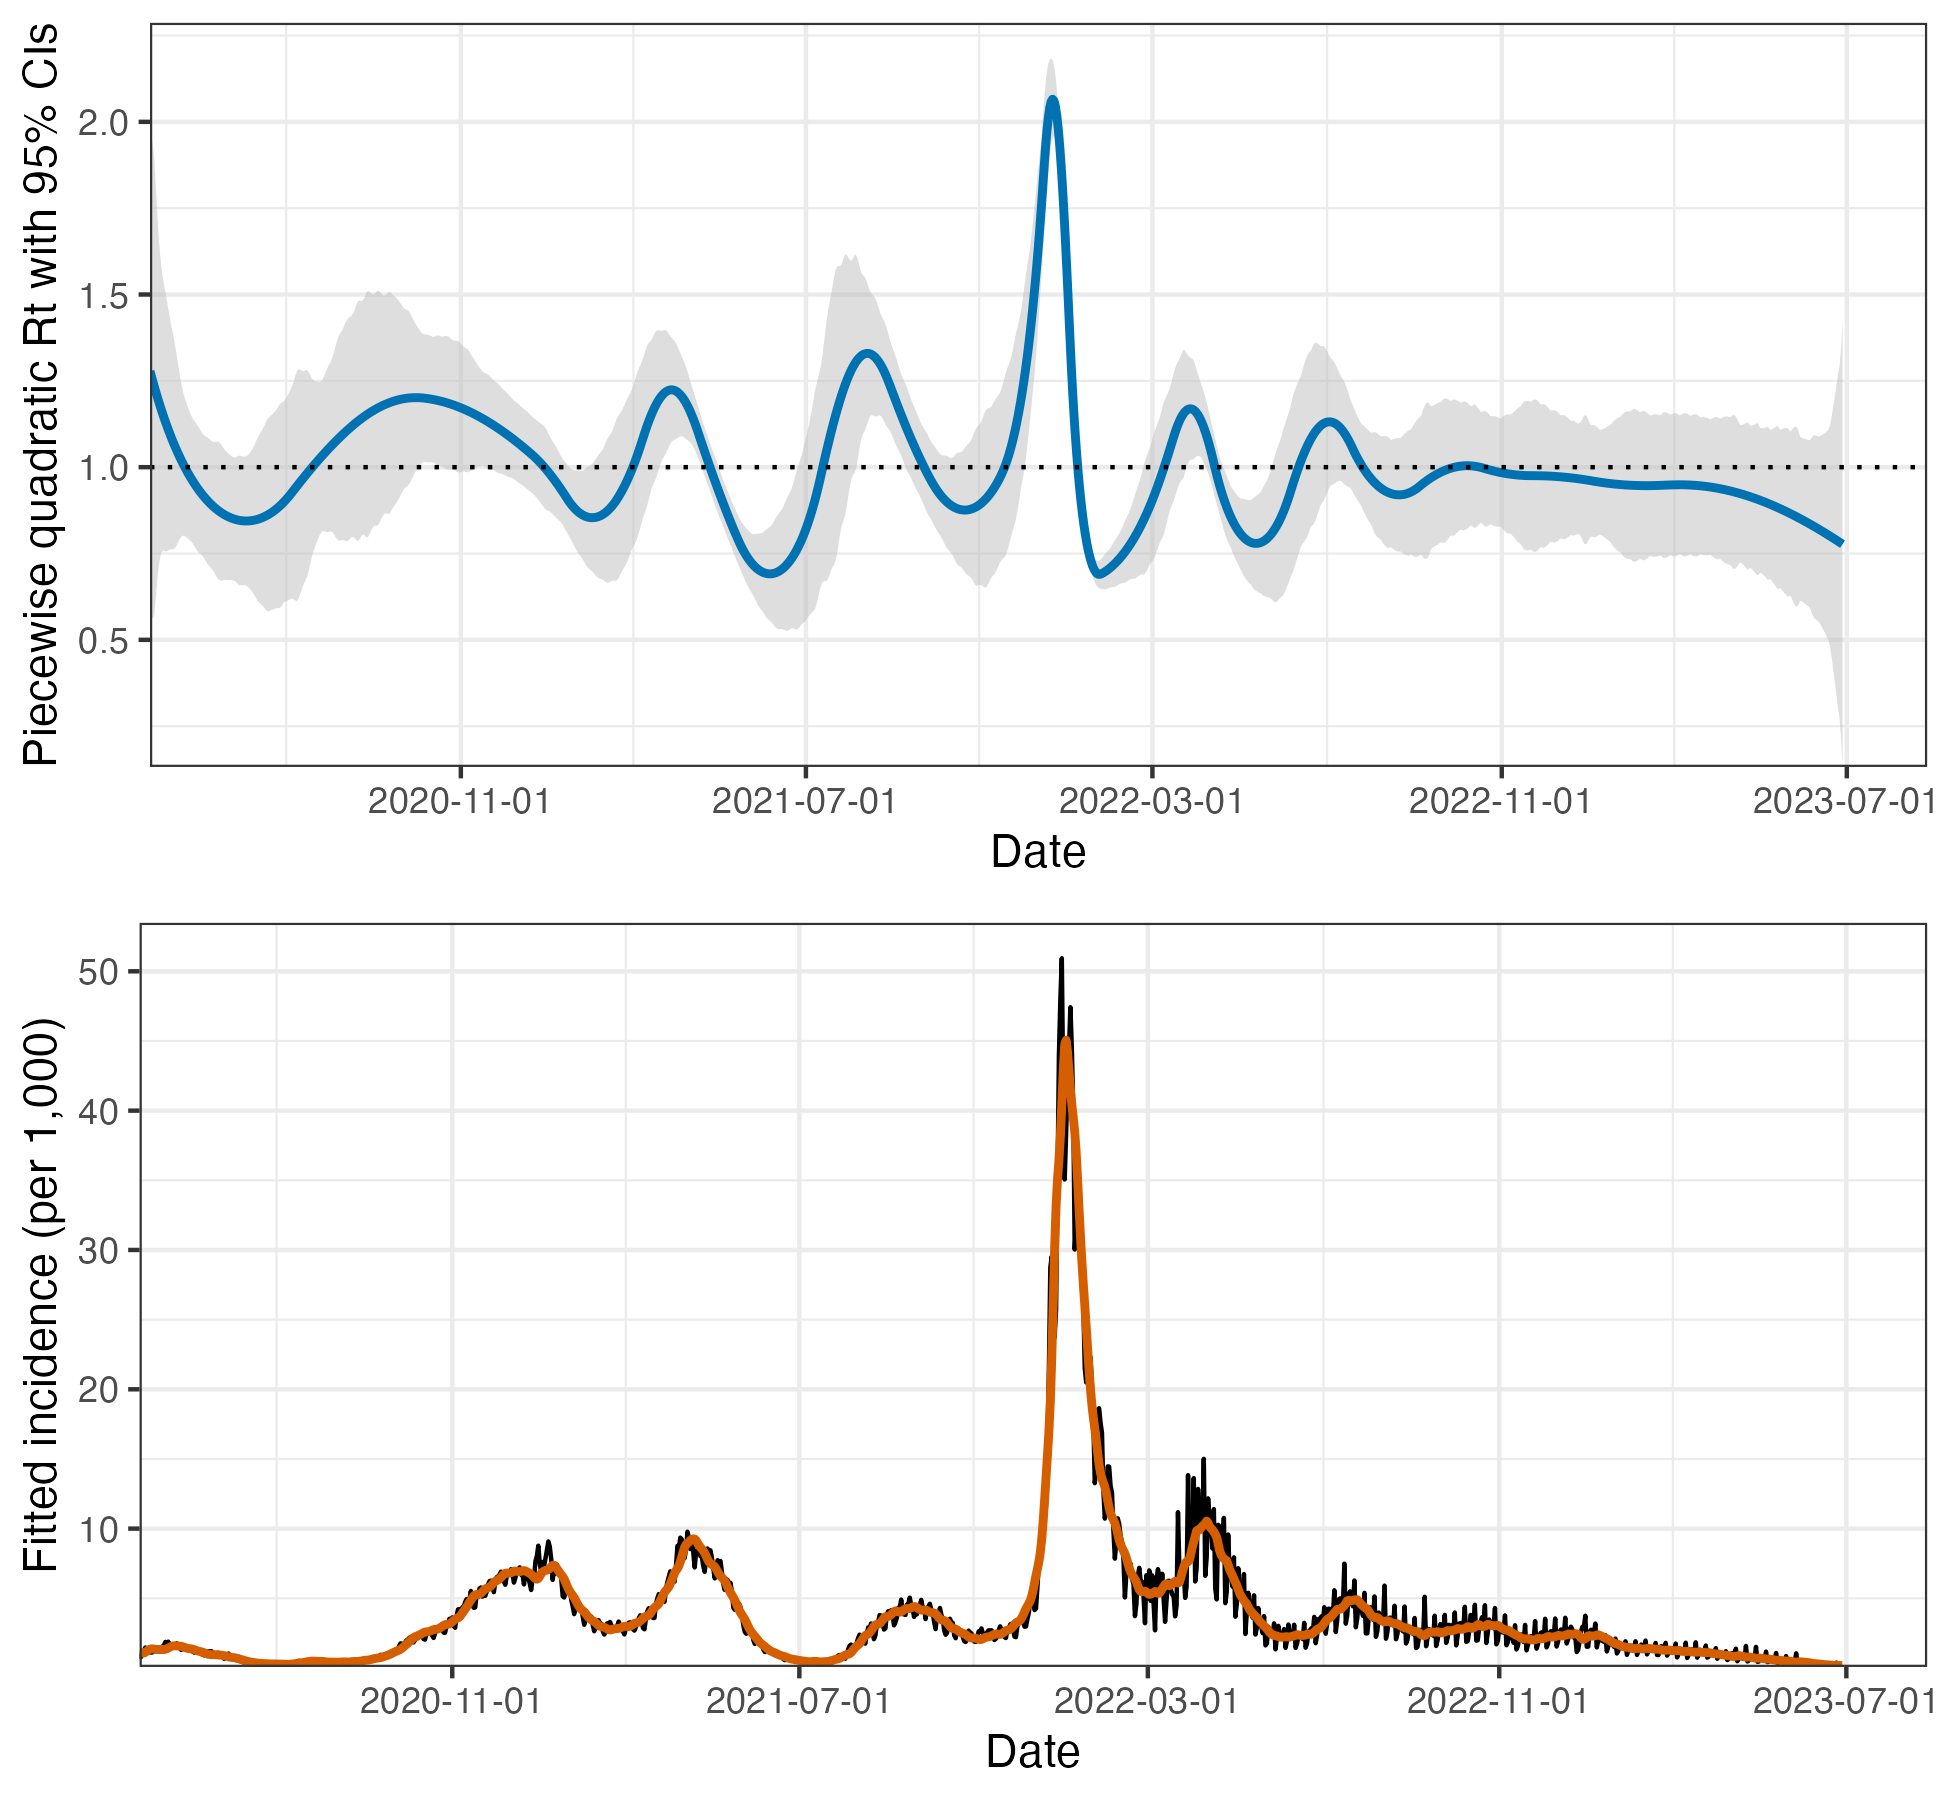
\includegraphics[width=.9\textwidth]{fig/intro-fig-new.png}
  \caption{A demonstration of effective reproduction number estimation 
  by \RtEstim\ and the corresponding fitted incident cases for the Covid-19 epidemic 
  in Canada during a period from March 28, 2020 to June 28, 2023. 
  The blue curve in the top panel is the estimated piecewise
  quadratic $\calR_t$ and the gray ribbon is the corresponding 95\% confidence band. 
  The black curve in the bottom panel is the observed Covid-19 daily confirmed 
  cases, and the orange curve is the fitted incidence 
  corresponding to the estimated $\calR_t$.}
  \label{fig:intro-fig}
\end{figure}

While our approach is straightforward and requires little domain knowledge for
implementation, we also implement a number of refinements. 
We use a proximal Newton method to solve the convex optimization problem along
with warm starts to produce estimates efficiently, typically in a matter of 
seconds, even for long sequences of data. In a number of simulation experiments, 
we show empirically that our approach is more accurate than existing methods at 
estimating the true effective reproduction numbers. 


The manuscript proceeds as follows. We first introduce the methodology of
\RtEstim\ including the usage of renewal equation and the development of Poisson
trend filtering estimator. We explain how this method could be interpreted from
the Bayesian perspective, connecting it to previous work in this context. We
provide illustrative experiments comparing our estimator to \EpiEstim\ and
\EpiLPS. We then apply our \RtEstim\ on the Covid-19 pandemic incidence in
British Columbia and the 1918 influenza pandemic incidence in the United States. 
Finally, we conclude with a discussion of the advantages and limitations of our 
approach and describe practical considerations for effective reproduction number
estimation.


\section{Methods}

\subsection{Renewal model for incidence data} 

The effective reproduction number $\calR(t)$
is defined to be the expected number of secondary infections at time $t$
produced by a primary infection sometime in the past.
To make this precise, denote the number of new infections at time $t$ 
as $y(t)$. Then the total primary infectiousness can be written as 
$\eta(t) := \int_0^{\infty} p(i) y(t-i) \diff i$, 
where $p(i)$ is the probability that a new secondary infection is the result
primary infection which occurred $i$ time units in the past. 
The reproduction number is then given as the value that equates
\begin{equation} \label{eq:pre-renew-equation}
  \bbE[y(t) \mid y(j),\ j<t]=\calR(t)\eta(t)=\calR(t)\int_0^\infty p(i)y(t-i)\diff i,
\end{equation}
otherwise known as the renewal equation. The period between primary and secondary
infections is exactly the generation time of the disease, but given real data,
observed at discrete times (say, daily) this delay distribution must be discretized
into contiguous time intervals,
say, $(0,1], (1,2], \dots$, which results in the sequence $\{p_i\}_1^\infty$
corresponding to observations $y_t$ and resulting in the
discretized version of \eqref{eq:pre-renew-equation},
\begin{equation} \label{eq:renew-equation}
  \bbE[y_t \mid y_1,\ldots,y_{t-1}]=\calR_t\eta_t=\calR_t\sum_{i = 0}^\infty p_i y_{t-i}.
\end{equation}
Many approaches to estimating $\calR_t$ rely on \eqref{eq:renew-equation} as
motivation for their procedures, among them, \EpiEstim\ \citep{cori2013new} 
and \texttt{EpiFilter} \citep{parag2021improved}. 


In most cases, it is safe to assume that infectiousness disappears beyond 
$\tau$ timepoints ($p_i = 0$ for $i > \tau$) so that the truncated integral 
of the generation interval distribution $\int_0^\tau p_i\diff i = 1$.
Generation time, however, is usually unobservable and tricky to estimate, so
common practice is to approximate it by the serial interval: the period between
the symptom onsets of primary and secondary infections. If the infectiousness
profile after symptom onset is independent of the incubation period (the period
from the time of infection to the time of symptom onset), then this
approximation is justifiable: the serial interval distribution and the
generation interval distribution share the same mean. However, other properties
may not be similarly shared, and, in general, the generation interval
distribution is a convolution of the serial interval distribution with the
distribution of the difference between independent draws from the delay
distribution from infection to symptom onset. See, for example,
\cite{gostic2020practical} for a fuller discussion of the dangers of this
approximation. Nonetheless, treating these as interchangeable is common
\citep{cori2013new} and doing otherwise is beyond the scope of this work. 
Additionally, we assume that the generation interval (and, therefore, the 
serial interval), is constant over time $t$. That is, the probability $p(i)$ 
depends only on the gap between primary and secondary infections and not on 
the time $t$ when the secondary infection occurs. For our methods, we will 
assume that the serial interval can be accurately estimated from auxiliary 
data (say by contact tracing, or previous epidemics) and we will take it as 
fixed, as is common in existing studies, e.g., 
\cite{cori2013new,abry2020spatial,pascal2022nonsmooth}.


The renewal equation in \eqref{eq:renew-equation} relates observable data
streams (incident cases) occurring at different time points to the reproduction
number given the serial interval. The fact that it depends only on the observed
incident counts makes it reasonable to estimate $\calR_t$. However, 
data collection idiosyncrasies can obscure this relationship. Diagnostic testing
targets symptomatic individuals, omitting asymptomatic primary infections which
can lead to future secondary infections. Testing practices, availability, and
uptake can vary across space and time \citep{pitzer2021impact,
hitchings2021usefulness}. Finally, incident cases as reported to public health
are subject to delays due to laboratory confirmation, test turnaround times, and
eventual submission to public health \citep{pellis2021challenges}. For these
reasons, reported cases are lagging indicators of the course of the pandemic.
Furthermore, they do not represent the actual number of new infections that
occur on a given day, as indicated by exposure to the pathogen. The assumptions
described above (constant serial interval distribution, homogenous mixing,
similar susceptibility and social behaviours, etc.) are therefore consequential.
That said, \eqref{eq:renew-equation} also provides some comfort about deviations
from these assumptions. If $y_t$ is scaled by a constant (in time) describing
the reporting ratio, then it will cancel from both sides. Similar arguments mean
that even if such a scaling varies in time, as long as it varies slowly relative
to the set of $p_i$ that are larger than 0, \eqref{eq:renew-equation} will be a
reasonably accurate approximation, so that $\calR_t$ can still be estimated well
from reported incidence data. Finally, even a sudden change in reporting ratio, 
say from $c_1$ for $i=1,\ldots,t_1$ to $c_2$ for $i>t_1$ would only result in 
large errors for $t$ in the neighbourhood of $t_1$ (where the size of this 
neighbourhood is again determined by the effective support of $\{p_i\}$). 
This robustness to certain types of data reporting issues partially justifies 
using \eqref{eq:renew-equation} to calculate $\calR_t$.


\subsection{Poisson trend filtering estimator} 

We use the daily confirmed incident cases $y_t$ on day $t$ to estimate the
observed infectious cases under the model that $y_t$ given previous incident
cases $y_{t-1},\ldots,y_1$ and a constant serial interval distribution follows a
Poisson distribution with mean $\Lambda_t$. That is, 
$$y_t \mid y_1,\ldots,y_{t-1} \sim \mathrm{Poisson}(\Lambda_t), \textrm{ where } 
\Lambda_t =  \calR_t\sum_{i=0}^{t-1}p_i y_{t-i} = \calR_t\eta_t.$$ 
Given a history of $n$ confirmed incident counts $\bfy = {(y_1,\ldots,y_n)}^\top$,
our goal is to estimate $\calR_t$. A natural approach is to maximize the
likelihood, producing the MLE:
\begin{equation} \label{eq:mle}
  \begin{split}
    \widehat{\calR} &= \Argmax{\calR \in \bbR_+^n} \bbP(\calR \mid \bfy,\ \bfp)
    = \Argmax{\calR \in \bbR^n_+} \prod_{t = 1,\dots,n} 
    \frac{e^{- \calR_t \eta_t} \lr{\calR_t \eta_t}^{y_t} }{y_t!}\\
    &= \Argmin{\calR\in\bbR^n_+} \frac{1}{n}\sum_{t = 1}^n \calR_t\eta_t - 
    y_t\log(\calR_t\eta_t).
  \end{split}
\end{equation}
This optimization problem, however, is easily seen to yield a one-to-one
correspondence between the confirmed cases and the effective reproduction, i.e.,
$\widehat{\calR}_t = y_t / \eta_t$, so that the estimated sequence
$\widehat{\calR}$ will have no significant graphical smoothness.


The MLE is an unbiased estimator of the true parameter $\calR_t$, but
unfortunately has high variance: changes in $y_t$ result in proportional changes
in $\widehat\calR_t$. To avoid this behaviour, and to match the intuition that
$\calR_t \approx \calR_{t-1}$, we advocate enforcing smoothness of the effective
reproduction numbers. This constraint will decrease the variance, and hopefully
lead to more accurate estimation of $\calR$, as long as the smoothness
assumption is reasonable. Smoothness assumptions are common (see e.g.,
\cite{parag2021improved} or \cite{gostic2020practical}), but the \emph{type}
of smoothness assumed is critical. \cite{cori2020package} imposes smoothness
indirectly by estimating $\calR_t$ with moving windows of of past observations.
The Kalman filter procedure of \cite{parag2021improved} would enforce in
$\ell_2$-smoothness ($\int_0^n {(\widehat{\calR}''(t))}^{2}\diff t < C$ for some
$C$), although the algorithm results in $\widehat{\calR}$ taking values over a
discrete grid. \cite{pascal2022nonsmooth} produces piecewise-linear
$\widehat{\calR}_t$, which turns out to closely relate to a special case of our
methodology. Smoother estimated curves will provide high-level information 
about the entire epidemic, obscuring small local changes in $\calR(t)$, but 
may also remove the ability to detect large sudden changes, such as those 
resulting from lockdowns or other major containment policies. 


We choose to implement smoothness by assuming that $\log(\calR(t))$ is a
piecewise polynomial of arbitrary degree. We specifically consider discrete
splines with various degrees of continuity. For example, $0\th$-degree discrete
splines are piecewise constant, the \first-degree curves are piecewise linear,
and \second-degree curves are piecewise quadratic. For $k\geq 1$, $k\th$-degree
discrete splines are continuous and have continuous discrete differences up to
degree $k-1$ at the knots. To achieve such smoothness, we regularize the size of
changes between adjacent effective reproduction numbers. Because $\calR_t > 0$,
we explicitly penalize the divided differences (discrete derivatives) of
neighbouring values of $\log(\calR_t)$. To achieve this, we penalize the
$\ell_1$ norm of the divided differences, which introduces sparsity into the
curvature, so that the estimates can have heterogeneous smoothness in different
periods of time. It is a more realistic setting compared to
homogeneous smoothness created by the squared $\ell_2$ norm. Using different
orders of divided differences result in estimated effective reproduction numbers
with different smoothness assumptions. 


To enforce smoothness of $\hat\calR_t$, we add a trend filtering penalty to
\eqref{eq:rt-ptf} \citep{kim2009ell_1, tibshirani2014adaptive, tibshirani2022divided, 
sadhanala2022exponential}.
Let $\theta := \log(\calR) \in \bbR^n$, so that $\Lambda_t =
\eta_t \exp(\theta_t)$, and $\log(\eta_t \calR_t) = \log(\eta_t) +
\theta_t$. For evenly spaced incident case data, we
write our estimator as the solution to the optimization problem
\begin{equation} 
  \label{eq:rt-ptf}
  \widehat{\calR} = \exp(\widehat{\theta}) \quad\textrm{where}\quad \widehat{\theta} 
  = \Argmin{\theta\in\bbR^n} \eta^\top \exp(\theta) - \bfy^\top \theta + \lambda 
  \snorm{D^{(k+1)} \theta}_1,
\end{equation}
where $\exp(\cdot)$ applies elementwise.
Here, $D^{(k+1)} \in \bbZ^{(n-k-1)\times n}$ is the $(k+1)\th$ order divided
difference matrix for any $k \in \{0,\ldots,n-1\}$. $D^{(k+1)}$ is defined 
recursively as $D^{(k+1)} = D^{(1)} D^{(k)}$, where 
$D^{(1)} \in \{-1,0,1\}^{(n-k-1)\times (n-k)}$ is a sparse matrix with diagonal band: 
$$D^{(1)} = \begin{pmatrix} 
  -1 & 1 &  & & \\ 
  & -1 & 1 & & \\ 
  & & \ddots & \ddots & \\
  & & & -1 & 1 
\end{pmatrix}.$$ 
The tuning parameter $\lambda$ balances data
fidelity with desired smoothness. When $\lambda=0$, the problem in
\eqref{eq:rt-ptf} reduces to the MLE in \eqref{eq:mle}. Larger tuning parameters
privilege the regularization term and yield smoother estimates. Finally, there
exists $\lambda_{\textrm{max}}$ such that any $\lambda \geq
\lambda_{\textrm{max}}$ will result in $D^{(k+1)} \widehat {\theta} = 0$ and
$\widehat{\theta}$ will be the Kullback-Leibler projection of $\bfy$ onto the
null space of $D^{(k+1)}$ (see \autoref{sec:candidate-set}).


For unevenly-spaced incidence data, the spacing between neighboring parameters
varies with the time between observations, and thus, the divided differences
must be adjusted by the times that the observations occur. Given observation
times $\bfx = {(x_1,\dots,x_n)}^\top$, for $k \geq 1$, define a $k\th$-order
diagonal matrix $$X^{(k)} = \diag \lr{\frac{k}{x_{k+1} - x_1},\ \frac{k}{x_{k+2}
- x_2},\ \cdots,\ \frac{k}{x_n - x_{n-k}} }.$$ Letting $D^{(\bfx,1)} := D^{(1)}$,
then for $k\geq 1$, the $(k+1)\th$-order divided difference matrix for unevenly
spaced data can be created recursively by
$D^{(\bfx, k+1)} := D^{(1)} X^{(k)} D^{(\bfx,k)}.$ No adjustment is required
for $k=0$. 


Due to the penalty structure, this estimator is locally adaptive,
meaning that it can potentially capture local changes such as the initiation of
control measures. \cite{abry2020spatial,pascal2022nonsmooth} considered only the
\second-order divided difference of $\calR_t$ rather than its logarithm. In
comparison to their work, our estimator (1) allows for arbitrary degrees of
temporal smoothness and (2) avoids the potential numerical issues of
penalizing/estimating positive real values. Furthermore, as we will describe
below, our procedure is computationally efficient for estimation over an entire
sequence of penalty strengths $\lambda$ and provides methods for choosing how
smooth the final estimate should be.


\subsection{Solving over a sequence of tuning parameters}
\label{sec:candidate-set}

We can solve the Poisson trend filtering estimator over an arbitrary sequence of 
$\lambda$ that produces different levels of smoothness in the estimated curves. 
We consider a candidate set $\boldsymbol{\lambda} = \{\lambda_m\}_{m=1}^M$, 
which is a strictly decreasing $\lambda$ sequence.


Let $D := D^{(k+1)}$ for simplicity in the remainder of this section. As
$\lambda \to\infty$, the penalty term $\lambda \snorm{D\theta}_1$ dominants the
Poisson objective, so that minimizing the objective is asymptotically equivalent
to minimizing the penalty term, which results in $\snorm{D\theta}_1 = 0$. In
this case, the divided differences of $\theta$ with order $k+1$ is always $0$,
and thus, $\theta$ must lie in the null space of $D$, that is,
$\theta\in\mathcal{N}(D)$. The same happens for any $\lambda$ beyond this
threshold, so define $\lambda_{\textrm{max}}$ to be the smallest $\lambda$ that
produces $\theta\in\mathcal{N}(D)$. It turns out that this value can be written
explicitly as $\lambda_{\textrm{max}} = \snorm{\lr{D^{\dagger}}^{\top} \lr{\eta
- y}}_{\infty},$ where $D^{\dagger}$ is the (left) generalized inverse of $D$
satisfying $D^{\dagger} D = I$. Therefore, we use $\lambda_1 =
\lambda_{\textrm{max}}$ and then choose the minimum $\lambda_M$ to be
$r\lambda_{max}$ for some $r \in (0,1)$ (typically $r=10^{-5}$). Given any
$M\geq 3$, we generate a sequence of $\lambda$ values to be equally spaced on
the log-scale between $\lambda_1$ and $\lambda_M$. 


\subsection{Choosing a final $\lambda$}
\label{sec:cv}

We estimate model accuracy over the candidate set through $K$-fold cross
validation (CV) to choose the best tuning parameter. Specifically, we divide
$\bfy$ (except the first and last observations) roughly evenly and randomly into
$K$ folds, estimate $\calR_t$ for all $\boldsymbol{\lambda}$ leaving one fold
out, and then predict the held-out observations. Model accuracy can be measured
by multiple metrics such as mean squared error $\mathrm{MSE}(\widehat{y},\ y) =
n^{-1}\snorm{\widehat{y} - y}_2^2$ or mean absolute error
$\mathrm{MAE}(\widehat{y},\ y) = n^{-1}\snorm{\widehat{y} - y}_1$, but we prefer
to use the deviance, to mimic the likelihood in \eqref{eq:mle}: $D\lr{y,\
\hat{y}} = \fr{n} \sum_{i=1}^n 2\lr{y_i \log(y_i) - y_i\log(\hat{y}_i) - y_i +
\hat{y}_i},$ where we define $0\log(0) = 0$. 


To estimate the sequence efficiently, the model is fitted sequentially by 
visiting each component of $\boldsymbol{\lambda}$ in order. The estimates 
produced with a larger $\lambda$ are used as the initial values (warm starts) 
for the next smaller $\lambda$. By solving through the entire sequence of tuning 
parameters, we have a better chance to achieve a better trade-off between bias 
and variance, and accordingly, improved accuracy relative to procedures examining 
one fixed value of $\lambda$. Note that for any $K$ and any $M$, we will end up 
estimating the model $(K+1)M$ times rather than once.


\subsection{Approximate confidence bands} 
\label{sec:conf-band} 

We also provide empirical confidence bands of the estimators with  
approximate coverage guarantees. 
Consider the related estimator $\widetilde{\calR}_t$ defined as
$$\widetilde{\calR} = \exp(\widetilde{\theta}) \quad\textrm{where}\quad
\widetilde{\theta} = \Argmin{\theta\in\bbR^n} \eta^\top \exp(\theta) - \bfy^\top
\theta + \lambda \snorm{D \theta}_2^2.$$ 
Let $\widetilde{\bfy} = \eta \circ \calR$, and then it can be shown (for example,
Theorem 2 in \cite{vaiter2017degrees}) that an estimator for
$\Var(\widetilde{\bfy})$ is given by $\big(\mathrm{diag}(\widetilde{\bfy}^{-2})
+ \lambda D^{\top} D\big)^{\dagger}.$ Finally, an
application of the delta method shows that $\Var(\widetilde{\bfy}_t) / \eta_t^2$
is an estimator for $\Var(\widetilde{\calR}_t)$ for each $t = 1, \cdots, n$. We
therefore use ${\big(\mathrm{diag}(\widetilde{\bfy}^{-2}) + \lambda
D^{\top} D\big)}^{\dagger}_t / \eta_t^2$ as an estimator
for $\Var(\widehat{\calR}_t)$. An approximate $(1-\alpha)\%$ confidence interval
then can be written as $\widehat{\calR}\pm \textrm{T}(\alpha/2,n-\textrm{df})s$, 
where $s_t$ is the square-root of $\Var(\widehat{\calR}_t)$ for each 
$t = 1, \cdots, n$ and $\textrm{df}$ is the number of changepoints in 
$\widetilde{\theta}$ plus $k+1$. 


\subsection{Bayesian perspective}

Unlike many other methods for $\calR_t$ estimation, our approach is frequentist
rather than Bayesian. Nonetheless, it has a corresponding Bayesian
interpretation: as a state-space model with Poisson observational noise,
autoregressive transition equation of degree $k\geq 0$, e.g., $\theta_{t+1} =
2\theta_t - \theta_{t-1} + \varepsilon_{t+1}$ for $k=1$, and Laplace transition
noise $\varepsilon_{t+1}\sim \mathrm{Laplace}(0,\ 1/\lambda)$. Compared to
\texttt{EpiFilter} \citep{parag2021improved},
 we share the same observational assumptions, but our approach has a
different transition noise. \texttt{EpiFilter} estimates the posterior
distribution of
$\calR_t$, and thus it can provide credible interval estimates as well. Our
approach produces the maximum \emph{a posteriori} estimate via an efficient
convex optimization, obviating the need for MCMC sampling. But the associated
confidence bands are created differently.


\section{Results}

Implementation of the our approach is provided in the \R\ package
\href{https://dajmcdon.github.io/rtestim/}{\texttt{rtestim}}. All experiments
are run in \R\ with version 4.3.1 on a MacBook with an Apple M1 Pro chip
and 32GB RAM running under macOS Sonoma 14.0. The \R\ packages used for
simulation and real-data application are versions \texttt{EpiEstim 2.2-4},
\texttt{EpiLPS 1.2.0}, and \texttt{rtestim 0.0.4}. 

\subsection{Simulation settings}

We simulate four scenarios of the time-varying effective reproduction numbers,
intended to mimic different epidemics. The first two scenarios are simple cases
that are rapidly controlled by intervention, where the graphical curves consist
of one discontinuity and two segments. Scenario 1 has constant $\calR_t$ before
and after an intervention, while Scenario 2 grows exponentially, then decays.
The other two scenarios are more complicated, where more waves in the epidemics
are involved. Scenario 3 has four linear segments with three discontinuities,
which reflect the effect of an intervention, resurgence to rapid transmission,
and finally suppression of the epidemic. Scenario 4 involves sinusoidal waves
throughout the epidemic.
The first three scenarios and the last scenario are motivated by
\cite{parag2021improved} and \cite{gressani2022epilps} respectively. 
We name the four scenarios as \textit{(1) piecewise constant}, \textit{(2) 
piecewise exponential}, \textit{(3) piecewise linear}, and \textit{(4) periodic} 
lines or curves respectively. 



In all cases, the times of observation are regular, and epidemics are of
length $n=300$. Specifically, in Scenario 1, $\calR_t = 2, 0.8$ before and after
$t=70$. In Scenario 2, $\calR_t$ increases and decreases exponentially with
rates $0.015, 0.005$ pre and post $t=50$. 
In Scenario 3, $\calR_t$ is piecewise linear with four discontinuous segments following 
\begin{align*}
    \calR(t) = & \lr{2.5 - \frac{0.5}{59}\lr{t-1}} \boldsymbol{1}_{[1,60]}(t)
     + \lr{0.8 - \frac{0.2}{49}\lr{t-61}} \boldsymbol{1}_{(60,110]}(t) \\
    & + \lr{1.7 + \frac{0.3}{39}\lr{t-111}} \boldsymbol{1}_{(110,150]}(t)
     + \lr{0.9 - \frac{0.4}{149}\lr{t-151}} \boldsymbol{1}_{(150,300]}(t),
\end{align*}
where $\boldsymbol{1}_{A}(t) = 1$, if $t\in A$, and $\boldsymbol{1}_{A}(t)=0$ otherwise. 
In Scenario 4, $\calR_t$ is realization of the
continuous, periodic curve generated by the function $$\calR(t) = 0.2 \big(
\lr{\sin(\pi t/12) + 1} + \lr{2 \sin\lr{\pi t / 6} + 2} + \lr{3
\sin(\pi t / 1.2) + 3}\big),$$ evaluated at equally spaced points $t\in [0,10]$. 
These settings are illustrated in the left column of Fig 2.


We assume that the serial interval follows Gamma distribution with fixed shapes
and scales $(3,3)$, $(2.5,2.5)$, $(3.5,3.5)$ and $(3.5,3.5)$ for Scenarios 1--4
respectively. We consider all epidemics starting from $y_1=2$ cases and
generating until timepoints $t=300$. We compute the expected incidence
$\Lambda_t$ using the renewal equation, and generate the incidence samples from
the Poisson distribution $y_t\sim \textrm{Pois}(\Lambda_t)$. To verify the
performance of our model under the violation of this distributional assumption
of incidence, we also generate incidence samples using the negative Binomial
distribution with dispersion size 5, i.e., $y_t\sim \textrm{NB}(\Lambda_t,
\textrm{size}=5)$. We generate 50 random samples for each setting of
experiments, resulting in 400 total experiments. An example of each effective
reproduction number scenario with a single corresponding Poisson and negative
Binomial sample incidence sequences is displayed in \autoref{fig:samples}. 

\begin{figure}[!h]
  \centering
  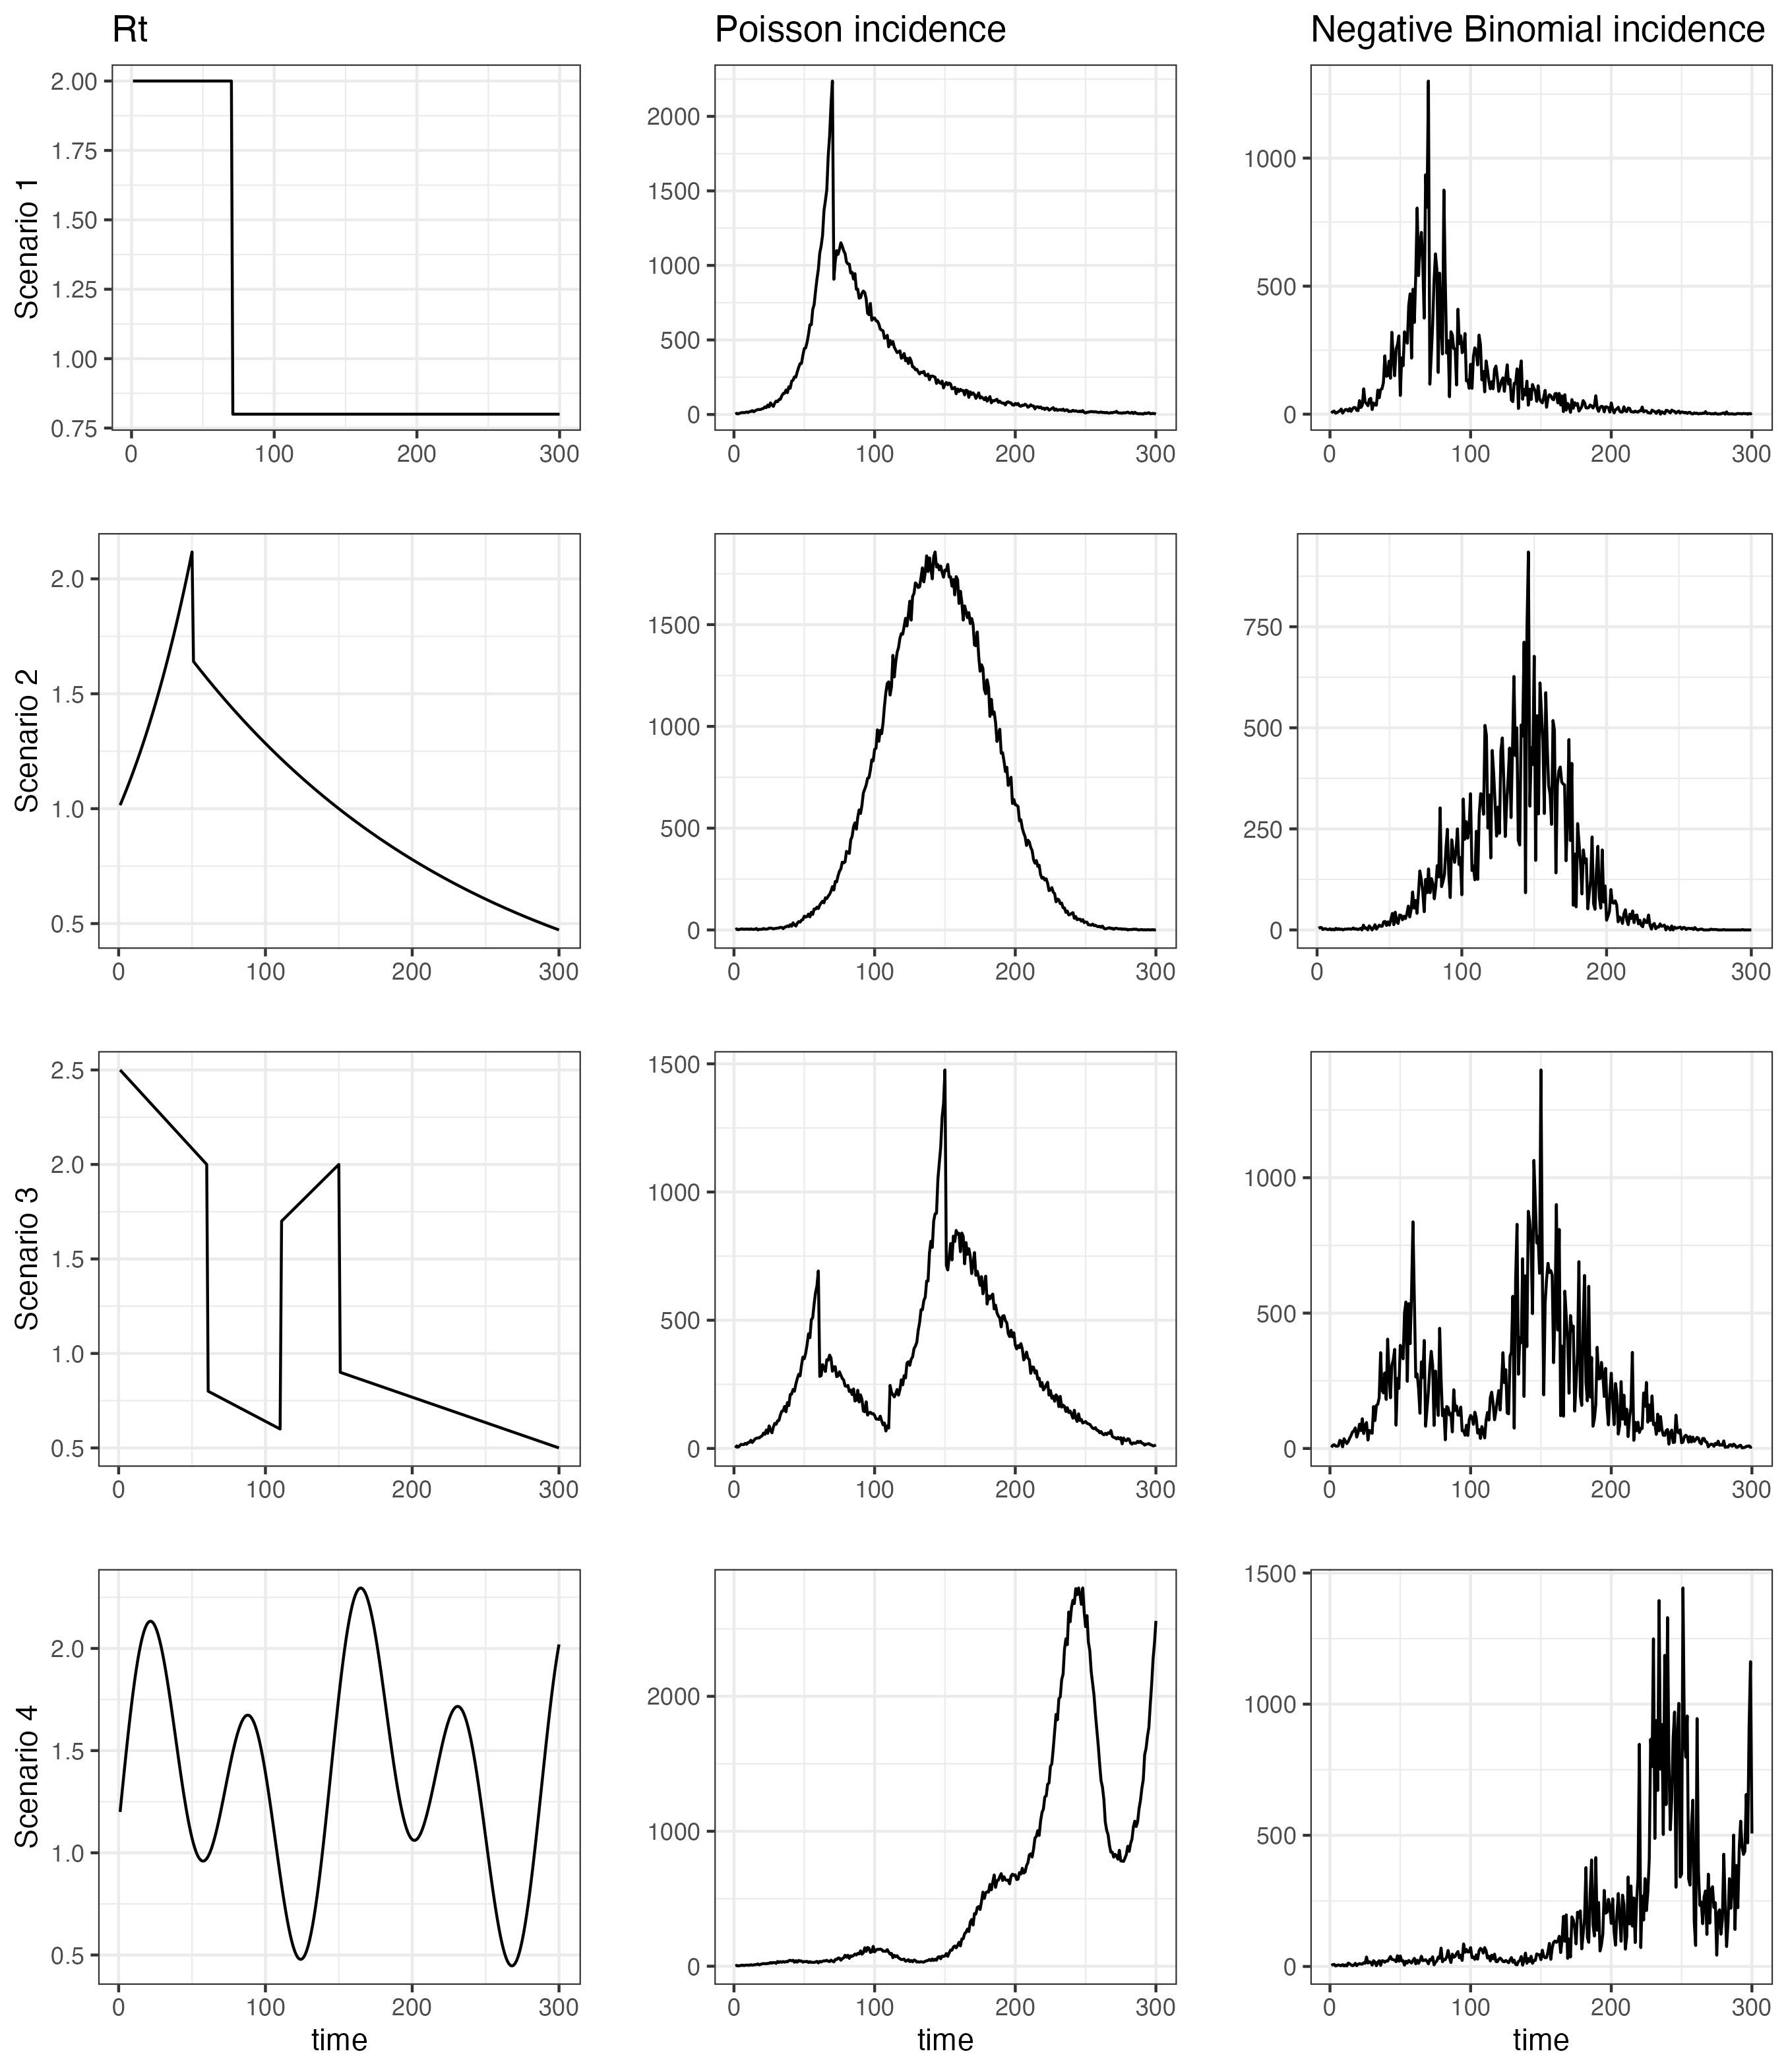
\includegraphics[width=.8\textwidth]{fig/plot_samples.png}
  \caption{The effective reproduction numbers (left column) and corresponding
  sample incident cases drawn from a  Poisson (middle column) or negative
  Binomial (right column) distribution. The rows correspond to the four
  $\calR_t$ settings.} 
  \label{fig:samples}
\end{figure}

We compare \RtEstim\ to \EpiEstim\ and \EpiLPS. Unfortunately,
\texttt{EpiFilter} frequently fails to converge due to the large case counts in
many simulations. \EpiEstim\ estimates the posterior distribution of effective
reproduction numbers given a Gamma prior and Poisson distributed incidence. It
estimates the reproduction number over a sliding window, assuming the
reproduction number is constant during the specific time window. A longer
sliding window averages out more fluctuations, leading to smoother estimates,
whereas, a shorter sliding window is more responsive to sudden spikes or
declines. We tried the default, a weekly sliding window, as well as a monthly
window. However, since neither considerably outperforms the other across all
scenarios, we defer the monthly case to the Appendix. \EpiLPS\ is another
Bayesian approach that estimates P-splines coupled with Laplace approximations
of the conditional posterior based on the negative Binomial likelihood. For
\RtEstim\ on the four scenarios respectively, we estimate (1) piecewise constant
$k=0$, (2) piecewise linear \& cubic $k=1,3$, (3) piecewise linear $k=1$ and (4)
piecewise cubic polynomials $k=3$. In each case, we examine a grid of 50
$\lambda$ values, selecting the best using 10-fold cross validation. 
For all models and problems, we use the serial interval distribution used to 
create the data. 


To measure estimation accuracy, we compare $\widehat{\calR}$ to $\calR$ using
the Kullback-Leibler (KL) divergence: a standard metric that measures the
distance between two probability distributions. Since $\calR_t$ can be regarded
as the expectation of Poisson distribution, we use the KL divergence for
Poisson distributions (averaged across all coordinates) to measure the accuracy
of the $\calR_t$ estimates 
$$D_{KL}(\calR \parallel \widehat{\calR}) = \sum_{t=1}^n w_t \lr{\calR_t 
\log\left(\frac{\calR_t} {\widehat{\calR}_t}\right) + \widehat{\calR}_t - {\calR}_t},$$ 
where $\calR = \left\{ \calR_t \right\}_{t=1}^n$ and 
$w_t = \eta_t / \sum_t \eta_t$ is the rescaled total infectiousness.
To fairly compare across methods, we drop the estimates during the first
week because estimates from \EpiEstim\ do not begin until $t=8$ (using a weekly
window). KL divergence is more appropriate for measuring accuracy because it
connects directly to the Poisson likelihood used to generate the data, whereas
standard measures like the mean-squared error correspond to Gaussian data. This
has the effect of increasing the relative cost of mistakes when $\Lambda_t$ is 
small. Other details of the experimental settings are deferred to the Appendix. 


\subsection{Simulation results}

\RtEstim\ overall outperforms \EpiEstim\ and \EpiLPS\ in the experimental study.
\autoref{fig:kl-res} visualizes the KL divergence across the three models. Under
both Poisson and negative Binomial distributions, \RtEstim\ is easily the most
accurate across Scenarios 1 and 3: the median of KL divergence is much lower
and the boxes frequently fail to overlap indicating a better performance than
the other two methods across all 50 simulations. 
The advantage is less for the
negative Binomial case compared to the Poisson case, but still obvious. 
\RtEstim\ and \EpiLPS\ have similar performance in Scenarios 2 and 4. 
For the Poisson case, \RtEstim\ and \EpiLPS\ both have very small KL scores, which 
are very close to 0. In Scenario 4, \RtEstim\ is slightly better for Poisson and 
\EpiLPS\ is better for negative Binomial, but the boxes largely overlap each other. 
\EpiLPS\ has a slightly lower median and a smaller IQR in Scenario 2 for the 
negative Binomial case. The two degrees of \RtEstim\ used for Scenario 2 perform 
very close to each other for both distributions, which implies a low risk of 
model misspecification. We will examine a single realization of each experiment 
to investigate these global conclusions in more detail.

\begin{figure}[!h]
  \centering
  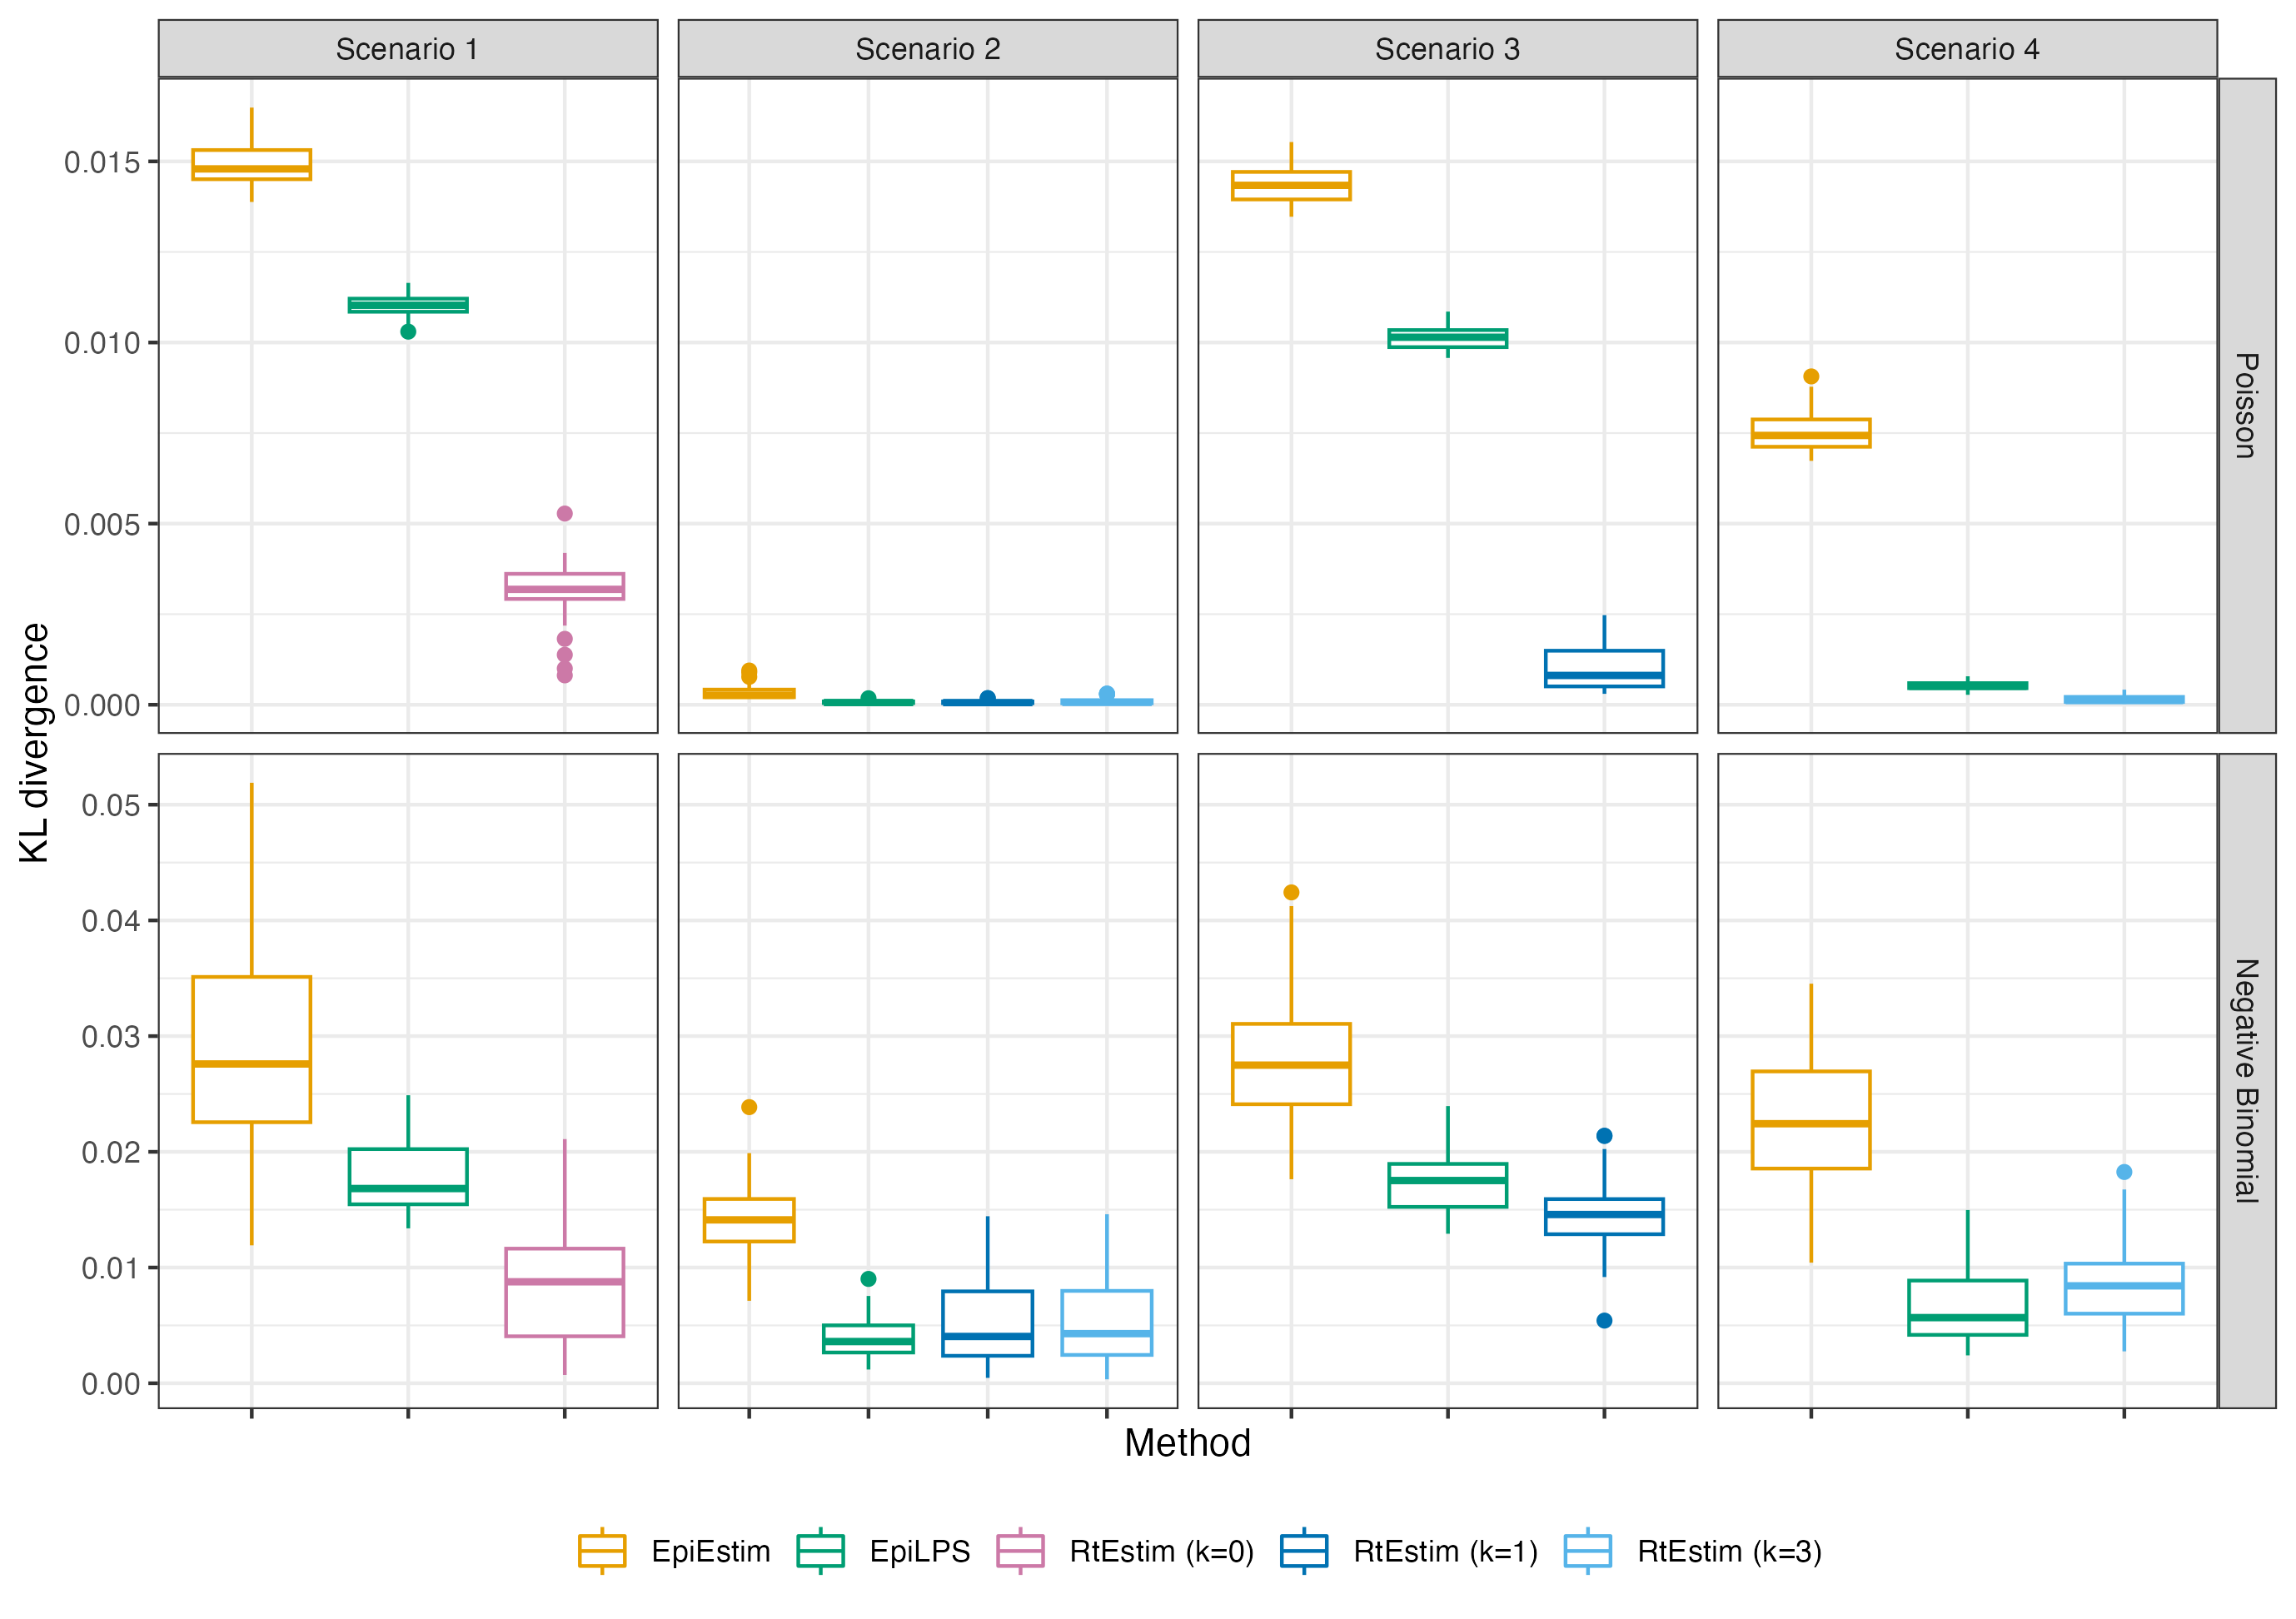
\includegraphics[width=.99\textwidth]{fig/KL_no_outlier.png}
  \caption{Boxplot of KL divergence between the estimated 
  $\hat{\calR}_t$ and the true $\calR_t$ across 50 random samples for 
  each approach given Poisson incidence \textit{(in top panels)} and negative 
  Binomial incidence \textit{(in bottom panels)} respectively.  
  Outliers are excluded. Full visualization is deferred to the Appendix.} 
  \label{fig:kl-res}
\end{figure}

\autoref{fig:pois-est} shows 1 realization for the estimated reproduction
numbers under the Poisson generative model for all 4 scenarios. Compared to
\EpiEstim\ and \EpiLPS, which have rather severe difficulties at the beginning
of the time series, \RtEstim\ estimates are more accurate --- they nearly overlap
with the true values --- without suffering from the edge problem. 
Scenario 2 presents an easy problem in terms of accurate estimation for all methods, 
except at the change point occurring at the end of the exponential growth. 
Although the truth is likely best represented with a piecewise cubic curve, the actual
curvature is so gentle that linear estimation ($k=1$) appears potentially
reasonable. We, therefore, fit piecewise linear and cubic $\hat{\calR}_t$ curves
using \RtEstim\ for Scenario 2 to evaluate model misspecification. 
However, \RtEstim\ with both degrees have difficulty recovering the acute rise 
in the growth phase. Due to this, \RtEstim\ has difficulty in convergence and 
can require more than $10^7$ iterates for all models across the $\lambda$ sequence 
and $10$-fold CV to converge in a couple of simulation samples. 
An explanation of such failure is that the model imposes discontinuity at the
changepoint, which hinders the estimates from fitting the two discontinuous
phases. Scenario 1 is the simplest case with only one knot and two constant
segments. Besides the edge problem, \EpiEstim\ and \EpiLPS\ produce ``smooth''
estimated curves that are continuous at the changepoint, which results in
large mistakes in that neighbourhood. Since the piecewise constant 
\RtEstim\ estimator does not force any smoothness in $\calR_t$, it easily 
captures the sharp change. 

\begin{figure}[!h]
  \centering
  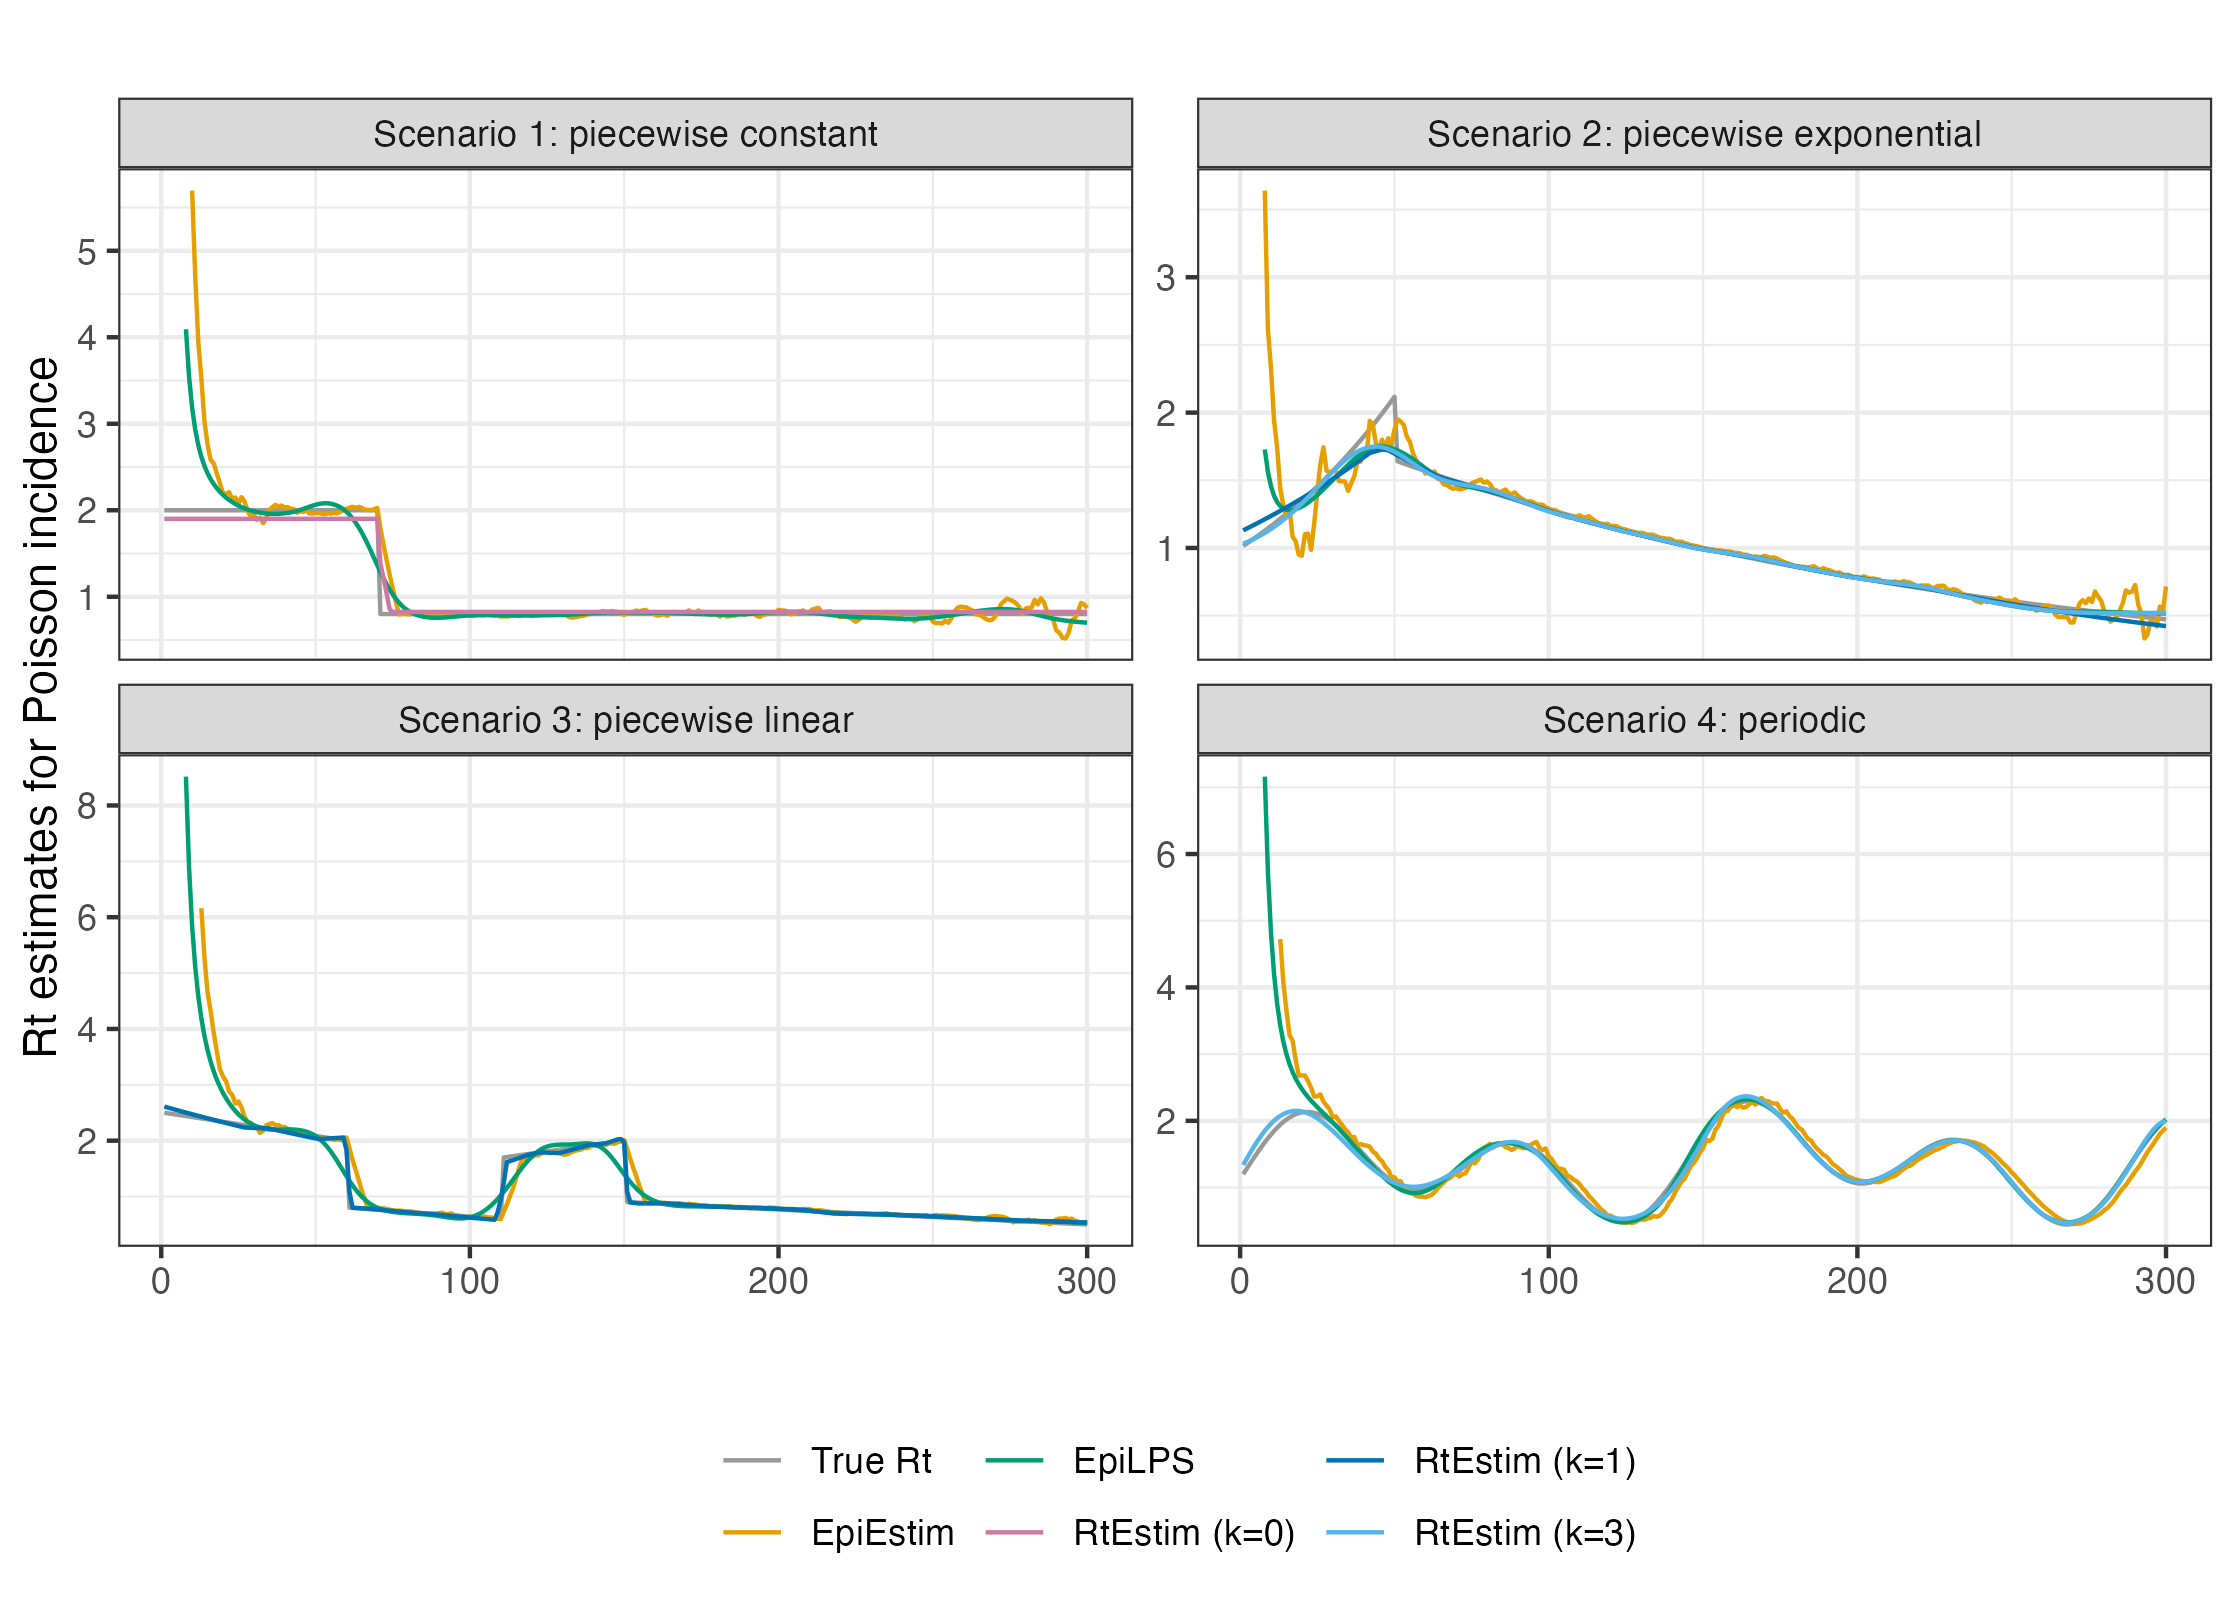
\includegraphics[width=.99\textwidth]{fig/Pois-res-plot.png}
  \caption{Example of effective reproduction number estimation for Poisson incidence.}
  \label{fig:pois-est}
\end{figure}

To investigate the performance under the violation of the Poisson distributional
assumption (of both \RtEstim\ and \EpiEstim), we also examine estimation
accuracy with negative Binomial data. \autoref{fig:nb-est} displays a
realization, analogous to the previous case, for all methods and scenarios.
\RtEstim\ has more difficulty relative to the Poisson incidence setting,
especially at the beginning of the outbreak. This is most pronounced in Scenario
4, where \RtEstim\ is overly smooth, except in the last wave. In Scenario 2,
\RtEstim\ successfully captures the changepoint, but suffers from the same
problem as in the Poisson setting. In Scenario 3, the piecewise linear \RtEstim\
recovers the curvature of $\calR_t$ well, but is less accurate than
in the Poisson incident cases.

\begin{figure}[!h]
  \centering
  \includegraphics*[width=.99\textwidth]{fig/NB-res-plot.png}
  \caption{Example of effective reproduction number estimation for negative Binomial
  incidence.}
  \label{fig:nb-est}
\end{figure}

Finally, it is important to provide a brief comparison of the running times of
three models across the $8$ experimental settings. We find that almost all
models across all experiments complete within $10$ seconds.
\RtEstim\ generally takes the longest, likely due to a relatively large
candidate set --- $50$ values of $\lambda$ and $10$ folds of cross validation --- 
while other models run only a single time for a fixed setting of hyperparameters 
per experiment. Additional results on timing comparisons are deferred to the
Appendix. 


\subsection{Real-data results: Covid-19 incident cases in British Columbia}

We implement \RtEstim\ on Covid-19 incident confirmed cases in British Columbia
(B.C.) as reported on May 18, 2023 (visualized in \autoref{fig:covid-data}) by
the B.C.\ Centre for Disease Control. 
We use the gamma distribution with shape $2.5$ and scale $2.5$
to approximate the serial interval function, which is empirically
reasonable, since they are close to the parameters in a recent study 
\citep{lehtinen2021relationship}, which summarizes estimated parameters of the 
serial interval distributions of SARS-CoV-2 by different approaches. 

\begin{figure}[!h]
  \centering
  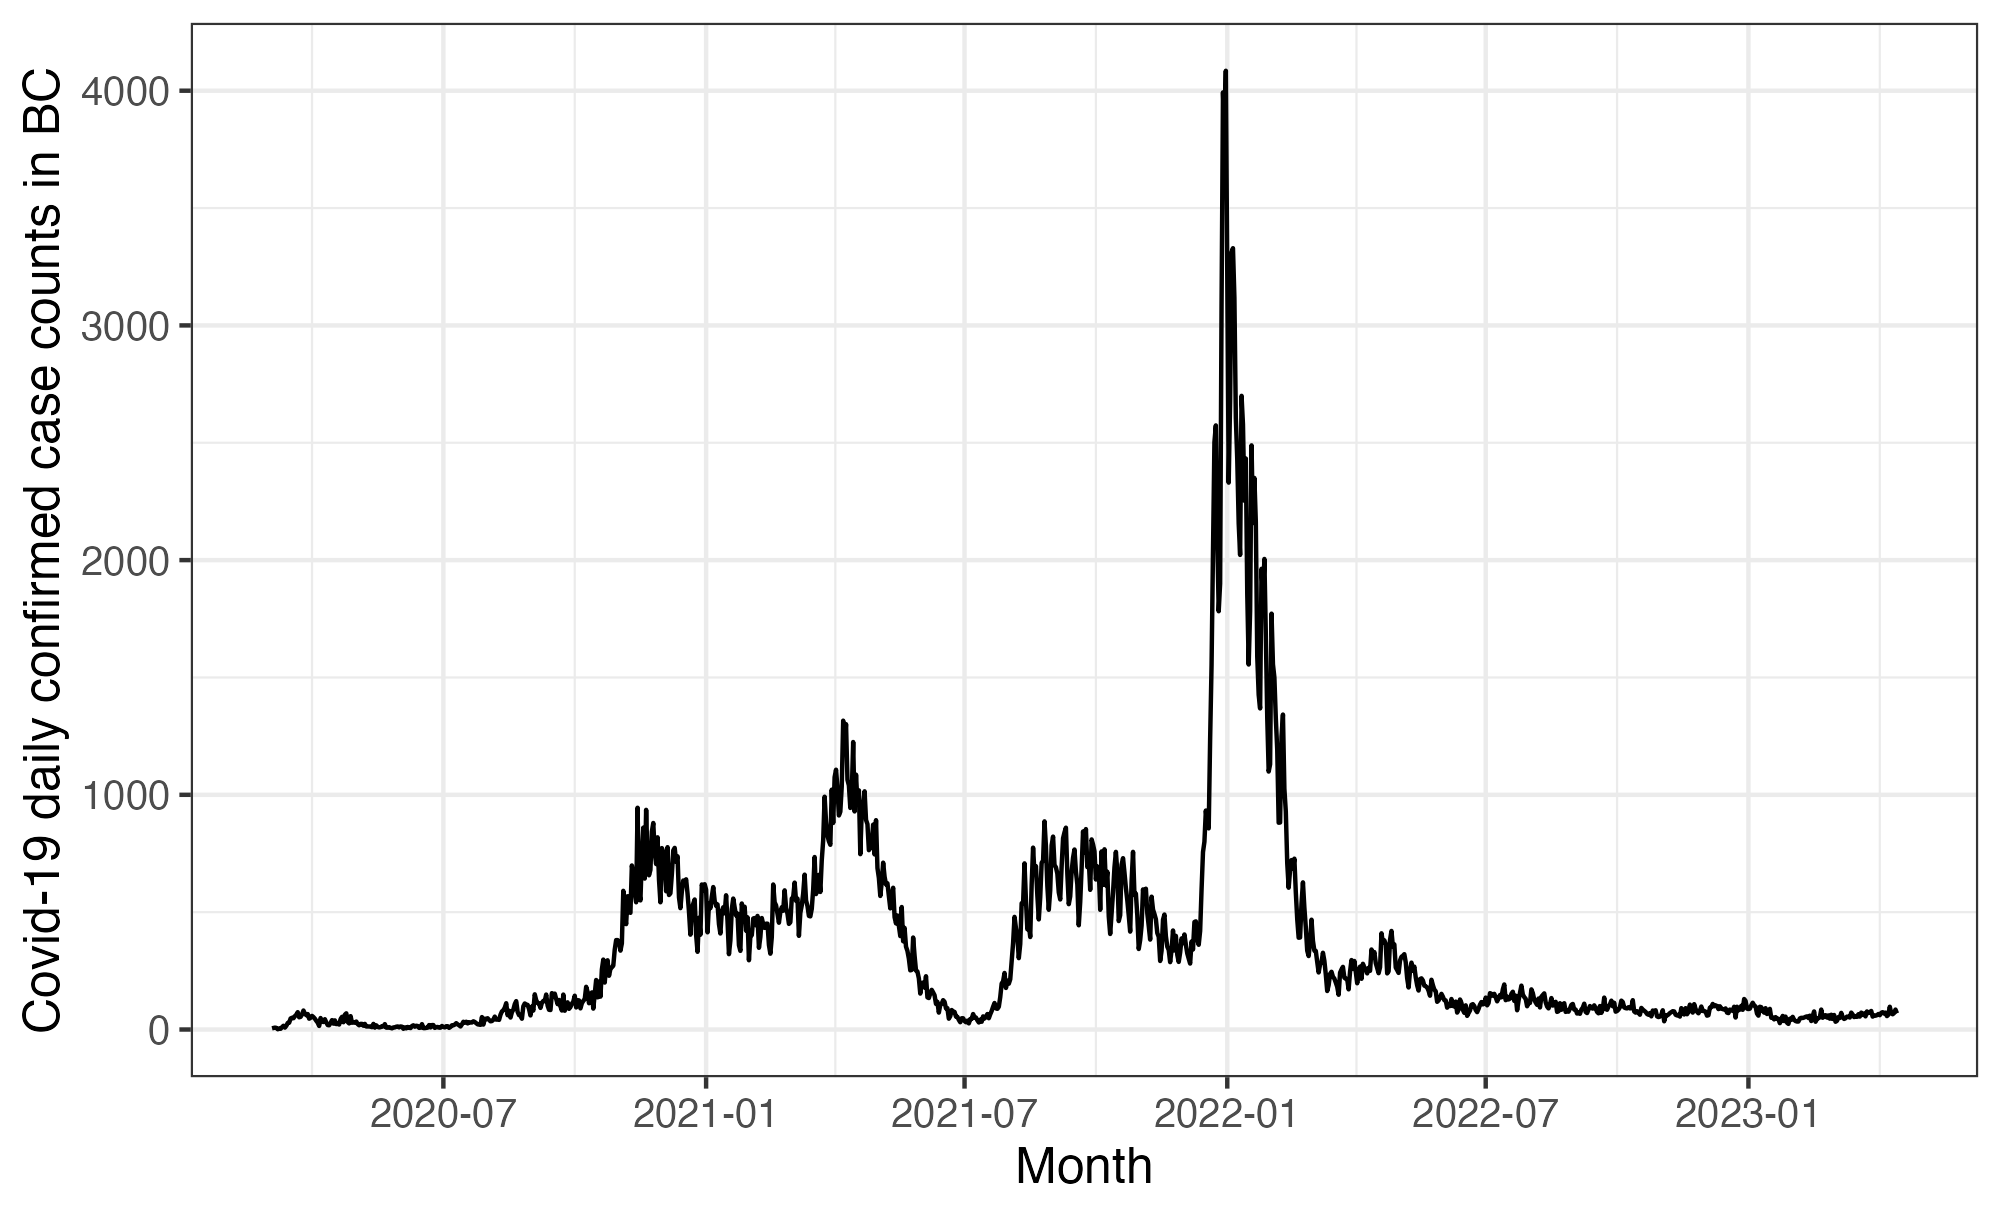
\includegraphics[width=0.9\textwidth]{fig/covid_dat.png}
  \caption{Covid-19 daily confirmed incident cases between March 1st, 
  2020 and April 15th, 2023 in British Columbia, Canada.} 
  \label{fig:covid-data}
\end{figure} 

Considering the first, second, and third polynomial degrees, the estimated 
effective reproduction numbers of Covid-19 in British Columbia
(illustrated in \autoref{fig:covid-rt}) are always less than $3$ except at the 
very early stage, which means that one distinct infected individuals on average 
infects less than three other individuals in the population. 
Examining three different settings for $k$, 
the temporal evolution of $\widehat{\calR}$ (across all regularization levels
$\lambda$) are similar near the highest peak around the end of 2021 before
dropping shortly thereafter. Throughout the estimated curves, the peaks and
troughs of the reproduction numbers precede the growth and decay cycles of
confirmed cases, as expected. We also visualize 95\% confidence bands for the
point estimates at the smallest one of the ``optimal'' tuning parameters with 
lowest CV (i.e., KL divergence) scores in \autoref{fig:covid-rt}.     

\begin{figure}[!h]
  \centering
  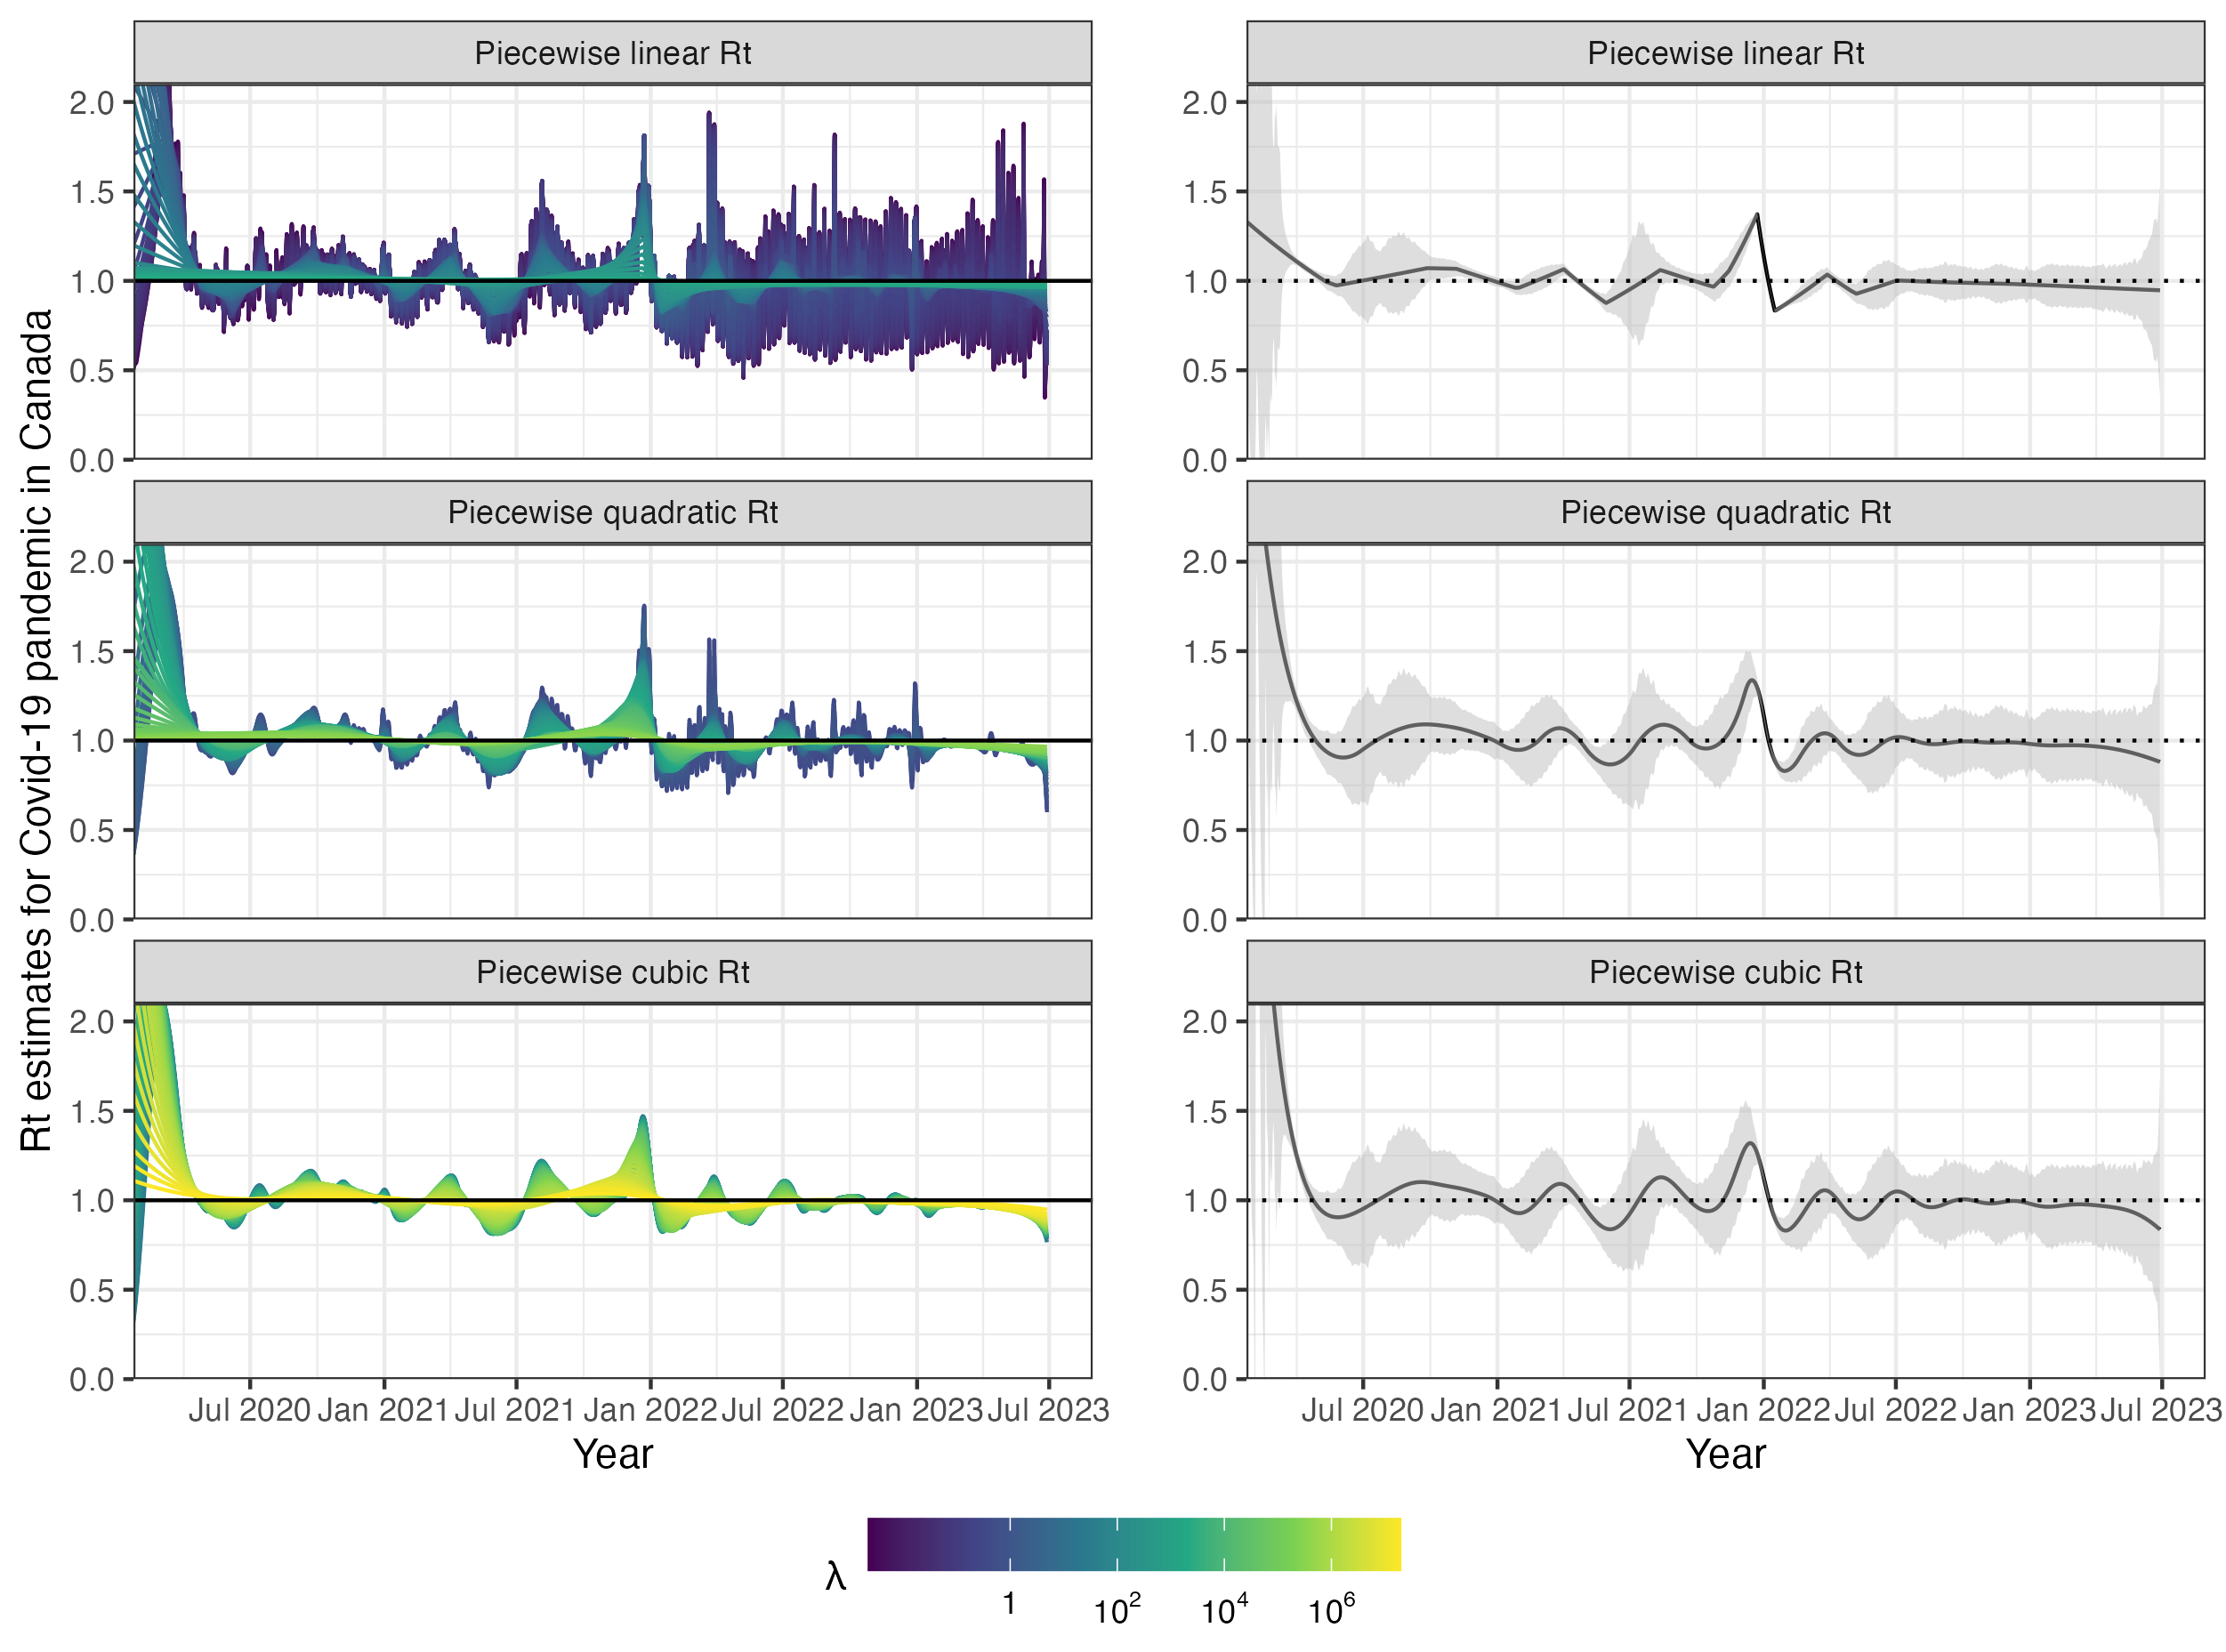
\includegraphics[width=0.9\linewidth]{fig/covid_full_res.png}
  \caption{Estimated effective reproduction numbers for Covid19 daily confirmed 
  counts between March 1st, 2020 and April 15th, 2023 in British Columbia, Canada. 
  The left panels demonstrate estimates corresponding to 50 tuning parameters. 
  The right panels display the CV-tuned estimates with 95\% confidence intervals. 
  The top, medium and bottom panels illustrate the estimated reproduction numbers 
  ($\calR_t$) using the Poisson trend filtering (in \eqref{eq:rt-ptf}) with 
  degrees $k=1,2,3$ respectively.} 
  \label{fig:covid-rt}
\end{figure} 

The estimated reproduction numbers are relatively unstable before April 1st,
2022. The highest peak coincides with the emergence and global spread of the
Omicron variant. The estimated reproduction numbers fall below 1 during two time
periods --- roughly from April 1st, 2021 to July 1st, 2021 and from January 1st,
2022 to April 1st, 2022. The first trough coincides with the introduction of
Covid-19 vaccines in British Columbia. The second trough, shortly after the
greatest peak may be due to variety of factors resulting in the depletion of the
susceptible population such as increased self-isolation in response to the peak
and media and immunity incurred via recent infection. Since around April 1st,
2022, estimated reproduction numbers have remained relatively stable
(fluctuating around $1$) corresponding to low reported cases (though reporting
behaviours have also changed significantly since the Omicron wave). 


\subsection{Real-data results: Pandemic influenza in Baltimore, Maryland, 1918}

We also apply \RtEstim\ to daily reported influenza cases in Baltimore, Maryland
occurring during the world-wide pandemic of 1918 from September to November. 
The dataset (shown in \autoref{fig:flu-dat}) is included in the \EpiEstim\ 
\R\ package. The 1918 influenza outbreak, caused by the H1N1 influenza A virus, 
was unprecedentedly deadly with case fatality rate over 2.5\%, infecting almost 
one-third of the population across the world \citep{taubenberger20061918}. 
The CV-tuned piecewise cubic estimates in \autoref{fig:flu-res} better capture 
the growth at the beginning of the pandemic in \autoref{fig:flu-dat}. 
The estimated $\calR_t$ curve suggests that the transmissibility of the pandemic 
grew rapidly over the first 30 days before declining below $1$ after 50 days. 
However, it also suggests an increase of the infectiousness toward the end of the 
period. With the currently available dataset, it is hard to tell if there is a 
next wave or a steady decline ahead. The CV-tuned piecewise constant and linear 
estimates in \autoref{fig:flu-res} both suggest a steady decline. This is supported 
by a couple of arguments. The influenza incidence reduces to $0$ in the end. 
The $\calR$ estimates of \EpiEstim\ with 1-week, 2-week and 4-week sliding windows 
in \cite{cori2013new} are all lower than the threshold $1$ in their right tails. 

\begin{figure}[!h]
  \centering
  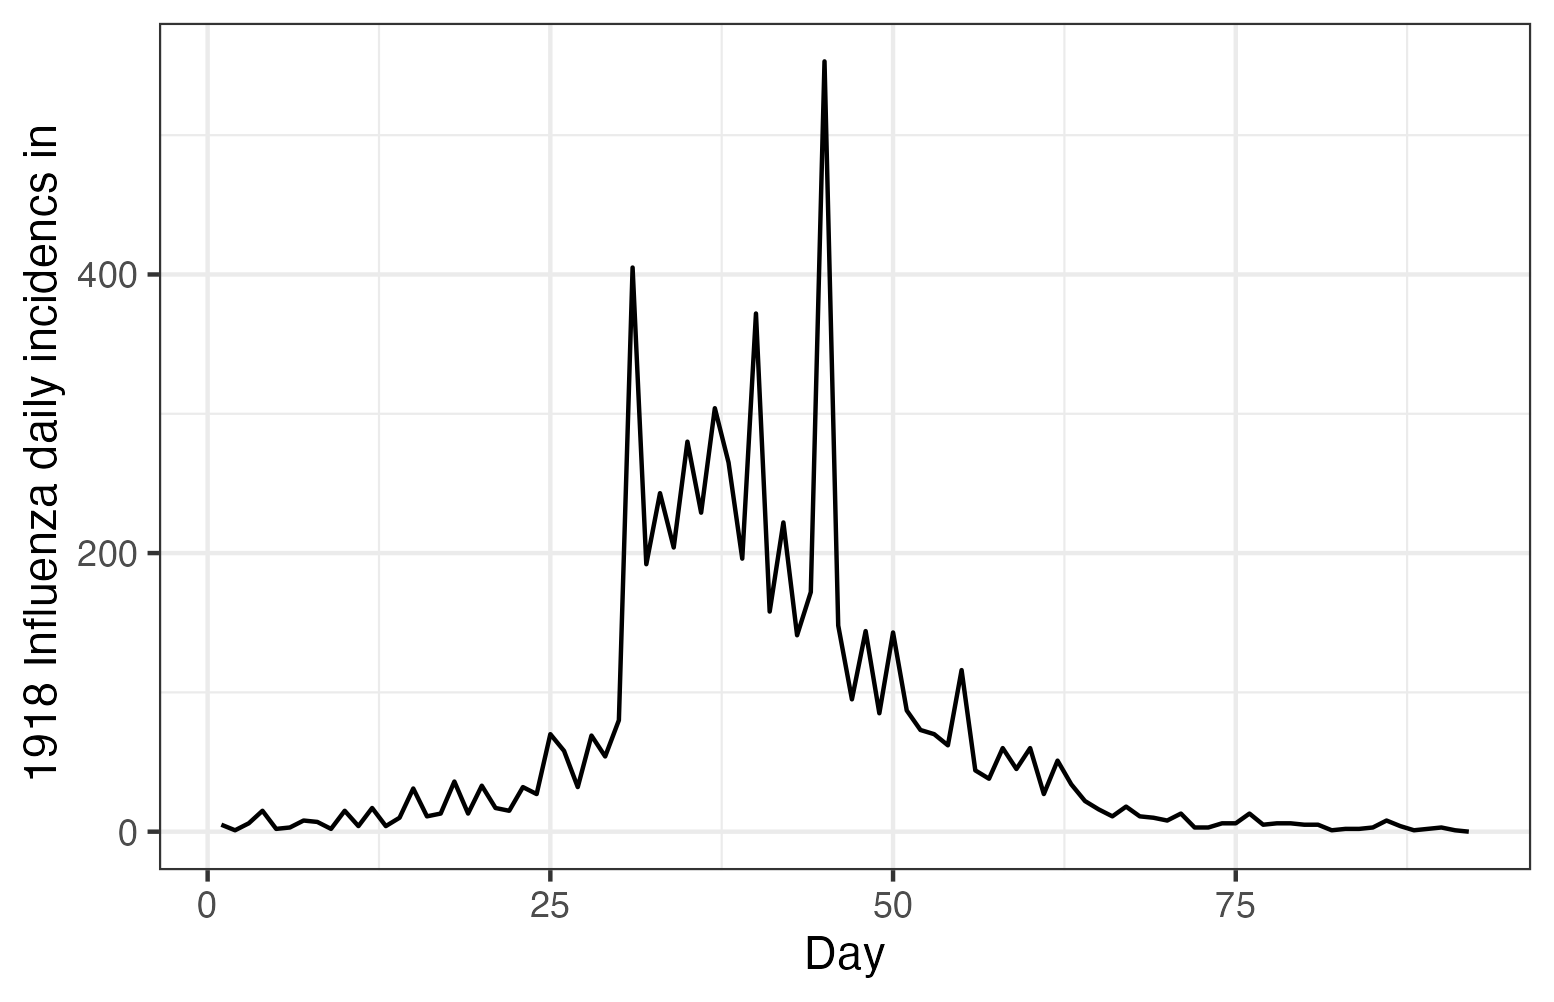
\includegraphics[width=0.9\linewidth]{fig/flu_dat.png}
  \caption{Daily influenza incident counts in Baltimore, Maryland between September 
  and November in 1918.} 
  \label{fig:flu-dat}
\end{figure} 

\begin{figure}[!h]
  \centering
  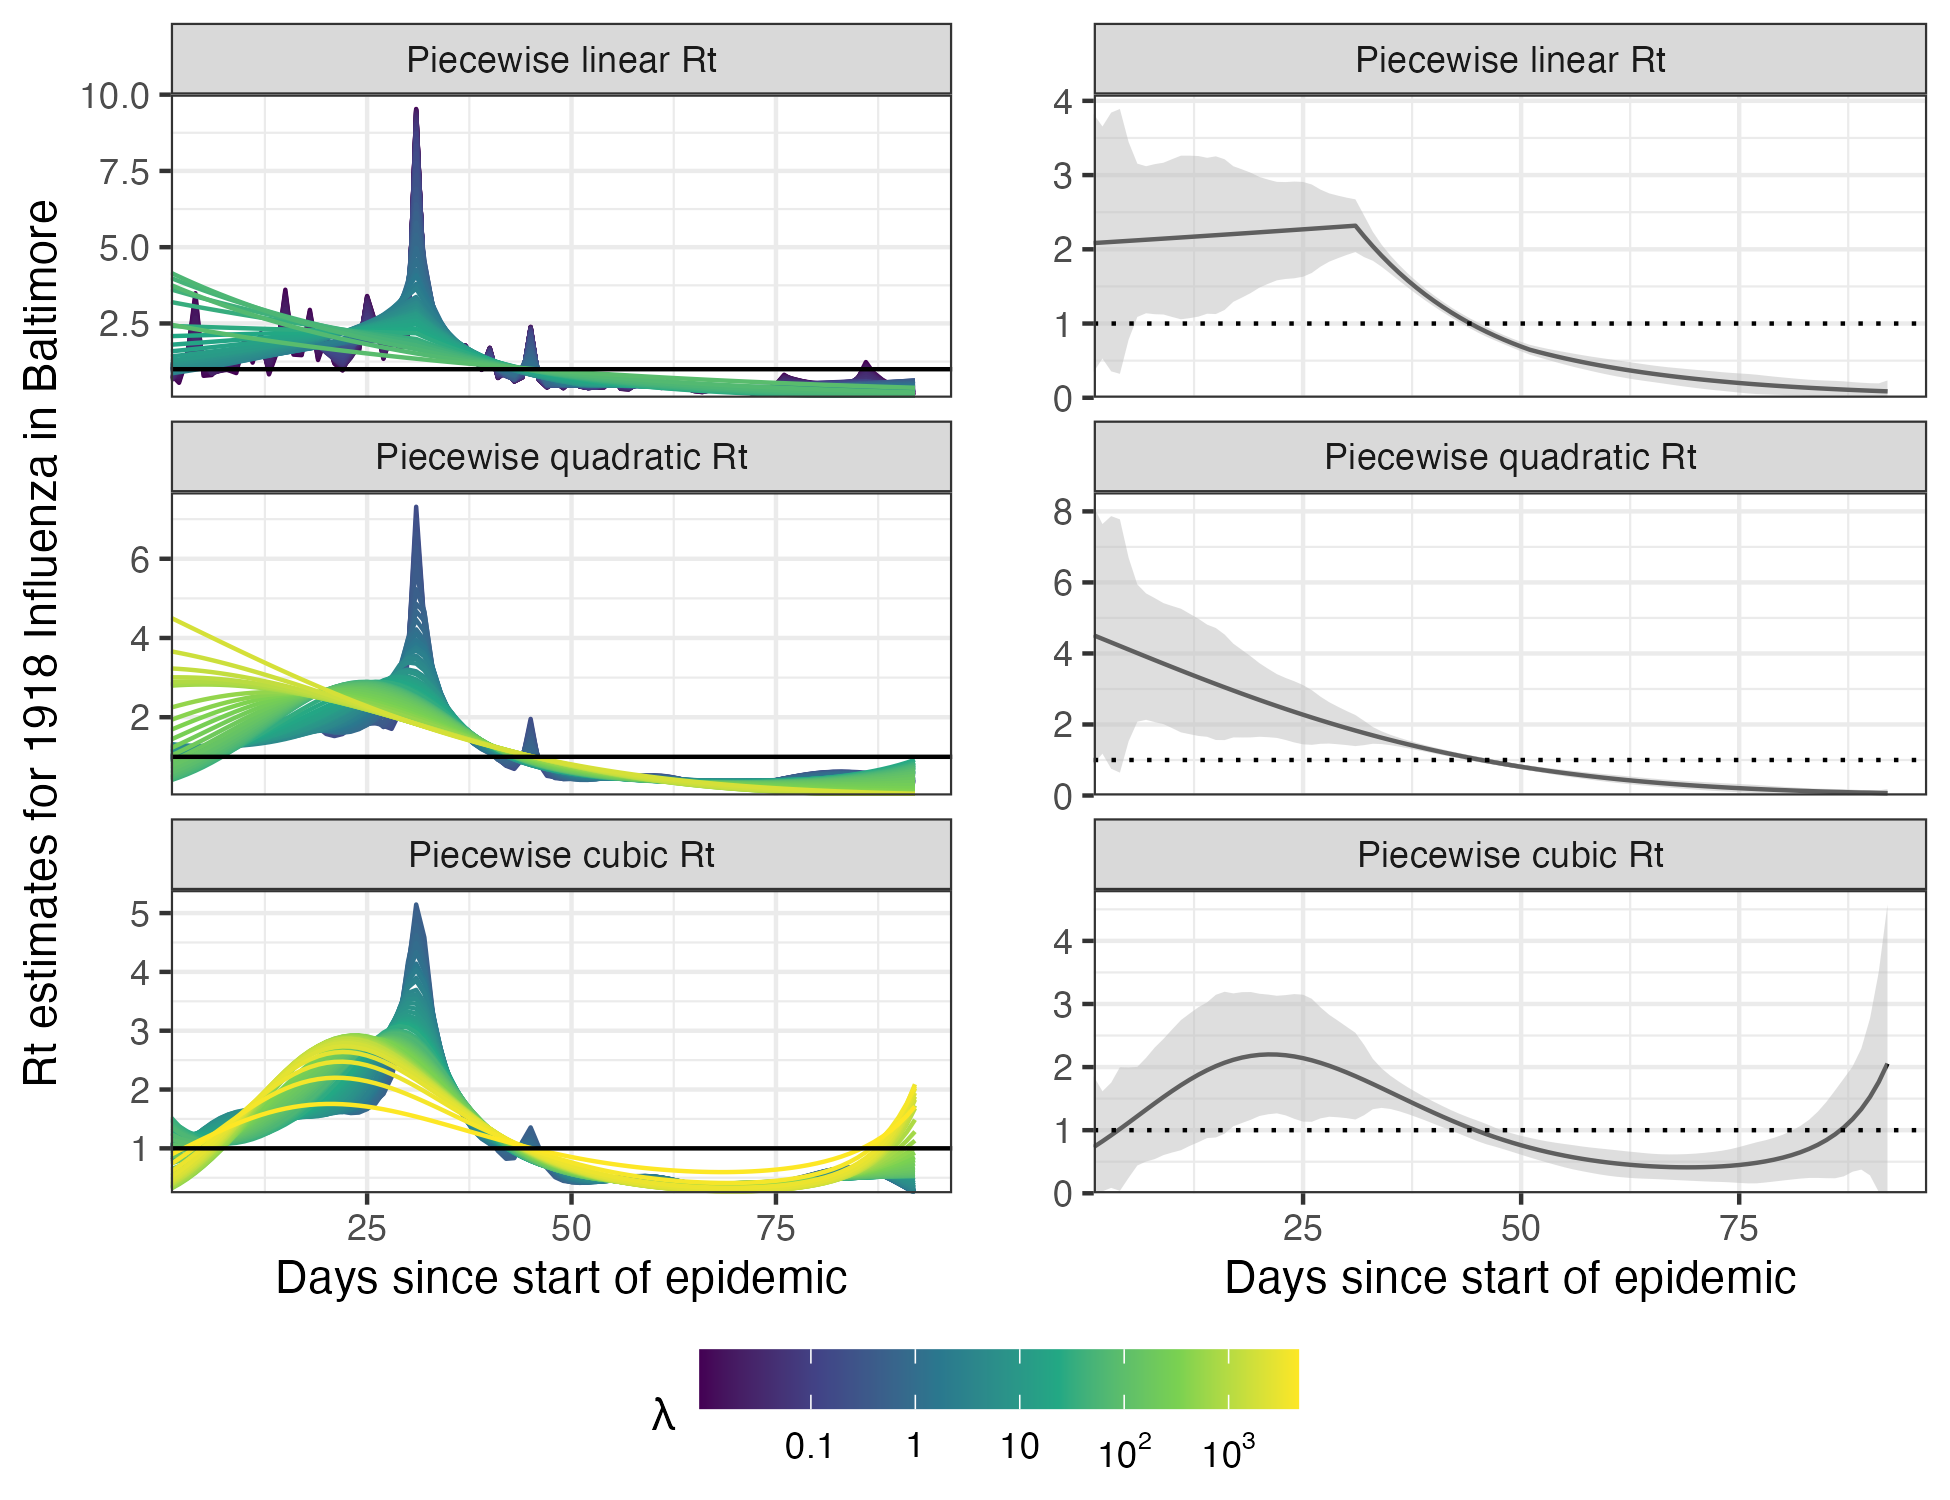
\includegraphics[width=0.9\linewidth]{fig/flu_full_res.png}
  \caption{Estimated effective reproduction numbers for influenza in
  Baltimore, Maryland in 1918. The left panels show estimates for all
  50 tuning parameters under consideration. The right column displays the 
  CV-tuned estimates with 95\% confidence bands. The rows (top to bottom) show
  estimated reproduction numbers ($\calR_t$) using the Poisson trend filtering
  (in \eqref{eq:rt-ptf}) with degrees $k=1,2,3$ respectively.} 
  \label{fig:flu-res}
\end{figure} 


\section{Discussion}

The \RtEstim\ methodology provides a locally adaptive estimator using Poisson
trend filtering on univariate data. It captures the heterogeneous smoothness of
effective reproduction numbers given observed incidence data rather than
resulting in global smoothness. This is a nonparametric regression model which
can be written as a convex optimization (minimization) problem. Minimizing the
distance (averaged KL divergence per coordinate) between the estimators and
(functions of) observations guarantees data fidelity while the penalty on divided
differences between pairs of neighbouring parameters imposes smoothness. The
$\ell_1$-regularization results in sparsity of the divided differences, which
leads to heterogeneous smoothness within certain periods of time. 


The property of local adaptivity (heterogenous smoothness) is useful to
automatically distinguish, for example, seasonal outbreaks from outbreaks driven
by other factors (behavioural changes, foreign introduction, etc.). Given a
well-chosen polynomial degree, the growth rates can be quickly detected, 
potentially advising public health to implement policy changes. The effective
reproduction numbers can be estimated retrospectively to examine the efficacy of
such policies, whether they result in $\calR_t$ falling below 1 or the speed of
their effects. The smoothness of $\calR_t$ curves (including the polynomial 
degrees and tuning parameters) should be chosen based on the purpose of the 
study in practice, e.g., epidemic forecasting may require a more wiggly curve 
that contains more fluctuation information, while retrospective studies that 
solely target on understanding of the pandemic may prefer a smoother curve 
with less important information smoothed out. 


Our method \RtEstim\ provides a natural way to deal with missing data, for
example, on weekends and holidays or due to changes in reporting frequency.
While solving the convex optimization problem, our method can be easily 
used to unevenly space or irregularly reported data. Computing the total
primary infectiousness is also easily generalized to irregular reporting by
modifying the discretization of the serial interval distribution. Additionally,
because the $\ell_1$ penalty introduces sparsity (operating like a median
rather than a mean), this procedure is relatively insensitive to outliers
compared to $\ell_2$ regularization.


There are a number of limitations that may influence the quality of
$\calR_t$ estimation. While our model is generic for incidence data, 
rather than tailored to any specific disease, it does assume that the 
generation interval is short relative to the period of data collection. 
More specialized methodologies would be required for diseases with long 
incubation periods such as HIV or Hepatitis. 
Our approach, does not explicitly model imported cases, nor distinguish between
subpopulations that may have different mixing behaviour. 
While the Poisson distribution is common, it does not handle overdispersion
(observation variance larger than the mean). The negative binomial distribution
is a good alternative, but more difficult to estimate in this context.
As described in the introduction section, justifying the expression for $\calR$ 
assumes that a relatively constant proportion of true infections is reported. 
However, if this proportion varies with time (say, due to change in surveillance
practices and testing recommendations), the estimates may be biased over this
window. A good example is that in early January 2022, during the height of the
Omicron wave, British Columbia moved from testing all symptomatic individuals to
testing only those in at-risk groups. The result was a sudden change that would
render $\calR_t$ estimates on either side of this time point incommensurable.


As currently implemented, \RtEstim\ uses a fixed serial interval throughout the
period of study, but as factors such as population immunity vary, the serial
interval may vary as well \citep{nash2023estimating}.  
Another issue relates to the equating serial and generation intervals (also
mentioned above). The serial interval distribution is generally
wider than that of the generation interval, because the serial interval
involves the convolution of two distributions, and is unlikely to actually
follow a named distribution like Gamma, though it may be reasonably well
approximated by one. Our implementation allows for an arbitrary distribution to
be used, but requires the user to specify the discretization explicitly,
requiring more nuanced knowledge than is typically available.
Pushing this analysis further, to accommodate other types of incidence data
(hospitalizations or deaths), a modified generation interval distribution would be
necessary, and further assumptions would be required as well. Or else, one would
first need to deconvolve deaths to infection onset before using our software.


Besides all the advantages and limitations of the methodology discussed above, 
our \RtEstim\ estimator can be implemented easily through a lightweight \R\ 
package \texttt{rtestim} and computed efficiently through the numerical algorithm, 
proximal Newton method developed in \cpp, especially for large-scale data. 
With accessible incident cases, prespecified serial interval distribution, and
chosen polynomial degrees, \RtEstim\ is able to produce accurate estimation 
of effective reproduction numbers and provide tuning parameter selection 
through a path algorithm. 


%\section*{Supporting information}
%
%% Include only the SI item label in the paragraph heading. Use the \nameref{label} command to cite SI items in the text.
%\paragraph*{Fig 1.}
%\label{fig:intro-fig}
%{\bf A demonstration of effective reproduction number estimation 
%by \RtEstim\ and the corresponding fitted incident cases for the Covid-19 epidemic 
%in Canada during a period from March 28, 2020 to June 28, 2023.}
%The blue curve in the top panel is the estimated piecewise
%quadratic $\calR_t$ and the gray ribbon is the corresponding 95\% confidence band. 
%The black curve in the bottom panel is the observed Covid-19 daily confirmed 
%cases, and the orange curve is the fitted incidence 
%corresponding to the estimated $\calR_t$.
%
%\paragraph*{Fig 2.}
%\label{fig:samples}
%{\bf The effective reproduction numbers (left column) and corresponding
%sample incident cases drawn from a Poisson (middle column) or negative
%Binomial (right column) distribution.} The rows correspond to the four
%$\calR_t$ settings.
%
%\paragraph*{Fig 3.}
%\label{fig:kl-res}
%{\bf Boxplot of KL divergence between the estimated 
%$\hat{\calR}_t$ and the true $\calR_t$ across 50 random samples for 
%each approach given Poisson incidence \textit{(in top panels)} and negative 
%Binomial incidence \textit{(in bottom panels)} respectively.}  
%Outliers are excluded. Full visualization is deferred to the \nameref{Appendix}.
%
%\paragraph*{Fig 4.}
%\label{fig:pois-est}
%{\bf Example of effective reproduction number estimation for Poisson incidence.}
%
%\paragraph*{Fig 5.}
%\label{fig:nb-est}
%{\bf Example of effective reproduction number estimation for negative Binomial
%incidence.}
%
%\paragraph*{Fig 6.}
%\label{fig:covid-data}
%{\bf Covid-19 daily confirmed incident cases between March 1st, 
%2020 and April 15th, 2023 in British Columbia, Canada.}
%
%\paragraph*{Fig 7.}
%\label{fig:covid-rt}
%{\bf Estimated effective reproduction numbers for Covid19 daily confirmed 
%counts between March 1st, 2020 and April 15th, 2023 in British Columbia, Canada.} 
%The left panels demonstrate estimates corresponding to 50 tuning parameters. 
%The right panels display the CV-tuned estimates with 95\% confidence intervals. 
%The top, medium and bottom panels illustrate the estimated reproduction numbers 
%($\calR_t$) using the Poisson trend filtering (in \eqref{eq:rt-ptf}) with 
%degrees $k=1,2,3$ respectively.
%
%\paragraph*{Fig 8.}
%\label{fig:flu-dat}
%{\bf Daily influenza incident counts in Baltimore, Maryland between September 
%and November in 1918.}
%
%\paragraph*{Fig 9.}
%\label{fig:flu-res}
%{\bf Estimated effective reproduction numbers for influenza in
%Baltimore, Maryland in 1918.} The left panels show estimates for all
%50 tuning parameters under consideration. The right column displays the 
%CV-tuned estimates with 95\% confidence bands. The rows (top to bottom) show
%estimated reproduction numbers ($\calR_t$) using the Poisson trend filtering
%(in \eqref{eq:rt-ptf}) with degrees $k=1,2,3$ respectively.
%
%\paragraph*{Appendix.}
%\label{Appendix}
%{\bf Supplementary details on methodology and experiments of effective 
%reproduction number estimation with trend filtering.} 


\section*{Acknowledgments}

xxx
\nolinenumbers

% Either type in your references using
% \begin{thebibliography}{}
% \bibitem{}
% Text
% \end{thebibliography}
%
% or
%
% Compile your BiBTeX database using our plos2015.bst
% style file and paste the contents of your .bbl file
% here. See http://journals.plos.org/plosone/s/latex for 
% step-by-step instructions.
% 
\begin{thebibliography}{10}

  \bibitem{cori2020package}
  Cori A, Cauchemez S, Ferguson NM, Fraser C, Dahlqwist E, Demarsh PA, et~al..
    {EpiEstim}: estimate time varying reproduction numbers from epidemic curves;
    2020.
  
  \bibitem{cori2013new}
  Cori A, Ferguson NM, Fraser C, Cauchemez S.
  \newblock A new framework and software to estimate time-varying reproduction
    numbers during epidemics.
  \newblock American Journal of Epidemiology. 2013;178(9):1505--1512.
  
  \bibitem{thompson2019improved}
  Thompson RN, Stockwin JE, van Gaalen RD, Polonsky JA, Kamvar ZN, Demarsh PA,
    et~al.
  \newblock Improved inference of time-varying reproduction numbers during
    infectious disease outbreaks.
  \newblock Epidemics. 2019;29:100356.
  
  \bibitem{nash2023estimating}
  Nash RK, Bhatt S, Cori A, Nouvellet P.
  \newblock Estimating the epidemic reproduction number from temporally
    aggregated incidence data: A statistical modelling approach and software
    tool.
  \newblock PLoS Computational Biology. 2023;19(8):e1011439.
  
  \bibitem{abbott2020estimating}
  Abbott S, Hellewell J, Thompson RN, Sherratt K, Gibbs HP, Bosse NI, et~al.
  \newblock Estimating the time-varying reproduction number of {SARS-CoV-2} using
    national and subnational case counts.
  \newblock Wellcome Open Research. 2020;5:112.
  
  \bibitem{EpiNow2}
  Abbott S, Funk S, Hickson J, Badr HS, Monticone P, Ellis P, et~al..
    epiforecasts/{EpiNow2}: 1.4.0 release; 2023.
  
  \bibitem{lison2023generative}
  Lison A, Abbott S, Huisman J, Stadler T.
  \newblock Generative {B}ayesian modeling to nowcast the effective reproduction
    number from line list data with missing symptom onset dates.
  \newblock arXiv preprint arXiv:230813262. 2023;.
  
  \bibitem{parag2021improved}
  Parag KV.
  \newblock Improved estimation of time-varying reproduction numbers at low case
    incidence and between epidemic waves.
  \newblock PLoS Computational Biology. 2021;17(9):e1009347.
  
  \bibitem{gressani2022epilps}
  Gressani O, Wallinga J, Althaus CL, Hens N, Faes C.
  \newblock EpiLPS: A fast and flexible {B}ayesian tool for estimation of the
    time-varying reproduction number.
  \newblock PLoS Computational Biology. 2022;18(10):e1010618.
  
  \bibitem{trevisin2023spatially}
  Trevisin C, Bertuzzo E, Pasetto D, Mari L, Miccoli S, Casagrandi R, et~al.
  \newblock Spatially explicit effective reproduction numbers from incidence and
    mobility data.
  \newblock Proceedings of the National Academy of Sciences.
    2023;120(20):e2219816120.
  
  \bibitem{abry2020spatial}
  Abry P, Pustelnik N, Roux S, Jensen P, Flandrin P, Gribonval R, et~al.
  \newblock Spatial and temporal regularization to estimate {COVID-19}
    reproduction number \emph{R(t)}: Promoting piecewise smoothness via convex
    optimization.
  \newblock PLoS ONE. 2020;15(8):e0237901.
  
  \bibitem{pascal2022nonsmooth}
  Pascal B, Abry P, Pustelnik N, Roux S, Gribonval R, Flandrin P.
  \newblock Nonsmooth convex optimization to estimate the {C}ovid-19 reproduction
    number space-time evolution with robustness against low quality data.
  \newblock IEEE Transactions on Signal Processing. 2022;70:2859--2868.
  
  \bibitem{pircalabelu2023spline}
  Pircalabelu E.
  \newblock A spline-based time-varying reproduction number for modelling
    epidemiological outbreaks.
  \newblock Journal of the Royal Statistical Society Series C: Applied
    Statistics. 2023;72(3):688--702.
  
  \bibitem{ho2023accounting}
  Ho F, Parag KV, Adam DC, Lau EH, Cowling BJ, Tsang TK.
  \newblock Accounting for the Potential of Overdispersion in Estimation of the
    Time-varying Reproduction Number.
  \newblock Epidemiology. 2023;34(2):201--205.
  
  \bibitem{azmon2014estimation}
  Azmon A, Faes C, Hens N.
  \newblock On the estimation of the reproduction number based on misreported
    epidemic data.
  \newblock Statistics in Medicine. 2014;33(7):1176--1192.
  
  \bibitem{gressani2021approximate}
  Gressani O, Faes C, Hens N.
  \newblock An approximate {B}ayesian approach for estimation of the
    instantaneous reproduction number under misreported epidemic data.
  \newblock Biometrical Journal. 2022;65(6):2200024.
  
  \bibitem{jin2023epimix}
  Jin S, Dickens BL, Lim JT, Cook AR.
  \newblock {EpiMix}: A novel method to estimate effective reproduction number.
  \newblock Infectious Disease Modelling. 2023;8(3):704--716.
  
  \bibitem{hettinger2023estimating}
  Hettinger G, Rubin D, Huang J.
  \newblock Estimating the instantaneous reproduction number with imperfect data:
    a method to account for case-reporting variation and serial interval
    uncertainty.
  \newblock arXiv preprint arXiv:230212078. 2023;.
  
  \bibitem{gostic2020practical}
  Gostic KM, McGough L, Baskerville EB, Abbott S, Joshi K, Tedijanto C, et~al.
  \newblock Practical considerations for measuring the effective reproductive
    number, \emph{R}$_t$.
  \newblock PLoS Computational Biology. 2020;16(12):e1008409.
  
  \bibitem{pitzer2021impact}
  Pitzer VE, Chitwood M, Havumaki J, Menzies NA, Perniciaro S, Warren JL, et~al.
  \newblock The impact of changes in diagnostic testing practices on estimates of
    {COVID-19} transmission in the {U}nited {S}tates.
  \newblock American Journal of Epidemiology. 2021;190(9):1908--1917.
  
  \bibitem{hitchings2021usefulness}
  Hitchings MD, Dean NE, Garc{\'\i}a-Carreras B, Hladish TJ, Huang AT, Yang B,
    et~al.
  \newblock The usefulness of the test-positive proportion of severe acute
    respiratory syndrome coronavirus 2 as a surveillance tool.
  \newblock American Journal of Epidemiology. 2021;190(7):1396--1405.
  
  \bibitem{pellis2021challenges}
  Pellis L, Scarabel F, Stage HB, Overton CE, Chappell LH, Fearon E, et~al.
  \newblock Challenges in control of {COVID-19}: short doubling time and long
    delay to effect of interventions.
  \newblock Philosophical Transactions of the Royal Society B.
    2021;376(1829):20200264.
  
  \bibitem{kim2009ell_1}
  Kim SJ, Koh K, Boyd S, Gorinevsky D.
  \newblock $\ell_1$ trend filtering.
  \newblock SIAM Review. 2009;51(2):339--360.
  
  \bibitem{tibshirani2014adaptive}
  Tibshirani RJ.
  \newblock Adaptive piecewise polynomial estimation via trend filtering.
  \newblock The Annals of Statistics. 2014;42(1):285--323.
  
  \bibitem{tibshirani2022divided}
  Tibshirani RJ.
  \newblock Divided differences, falling factorials, and discrete splines:
    Another look at trend filtering and related problems.
  \newblock Foundations and Trends{\textregistered} in Machine Learning.
    2022;15(6):694--846.
  
  \bibitem{sadhanala2022exponential}
  Sadhanala V, Bassett R, Sharpnack J, McDonald DJ.
  \newblock Exponential Family Trend Filtering on Lattices.
  \newblock arXiv preprint arXiv:220909175. 2022;.
  
  \bibitem{vaiter2017degrees}
  Vaiter S, Deledalle C, Fadili J, Peyr{\'e} G, Dossal C.
  \newblock The degrees of freedom of partly smooth regularizers.
  \newblock Annals of the Institute of Statistical Mathematics. 2017;69:791--832.
  
  \bibitem{lehtinen2021relationship}
  Lehtinen S, Ashcroft P, Bonhoeffer S.
  \newblock On the relationship between serial interval, infectiousness profile
    and generation time.
  \newblock Journal of the Royal Society Interface. 2021;18(174):20200756.
  
  \bibitem{taubenberger20061918}
  Taubenberger JK, Morens DM.
  \newblock 1918 {I}nfluenza: the mother of all pandemics.
  \newblock Emerging Infectious Diseases. 2006;17(1):69--79.
  
\end{thebibliography}

\end{document}
